\documentclass[11pt]{article}
\usepackage{comment}
\usepackage[margin=1in]{geometry}
\usepackage{amsmath}
\usepackage[numbers]{natbib}
\usepackage{amssymb}
\usepackage{mathtools}
\usepackage{verbatim}
\usepackage[utf8]{inputenc}
\usepackage[english]{babel}
\usepackage{graphicx}
\usepackage{parskip}
\usepackage{url}
\usepackage{wrapfig}
\usepackage{subcaption}
\usepackage{dcolumn}
\usepackage{setspace}
\usepackage{hyperref}
\usepackage{cleveref}

\onehalfspacing
%\setstretch{1.55}
%\pagestyle{headings}
%\pagestyle{myheadings}
%\markright{Brian Manzo\hfill Applied Qualifying Review 2020 \hfill}
\usepackage{fancyhdr}

\pagestyle{fancy}
\fancyhf{}
\lhead{Applied Qualifying Review Exam}
\rhead{Brian Manzo}
\rfoot{Page \thepage}

\title{Applied Qualifying Review Exam}
\author{Brian Manzo}
\date{May 15, 2020}



\begin{document}
%\vspace{-5cm}
\maketitle

%\begin{abstract}
%\textbf{Abstract.} 
%The abstract.
%\end{abstract}

\section{Introduction}\label{sec:intro}

The United States experienced an unprecedented decline in mortality in the 20th century due to massive improvements in public health, rapid technological development, and significant behavioral changes among Americans of all ages and social classes\cite{penn2016}.
The economist Robert Gordon attributes the improvement in quality of life and accompanying decline in mortality rate during the 20th century to a very specific type of economic growth, but is relatively pessimistic that we can continue these trends into the 21st century\cite{gordon2016}.
In fact, recent research on this topic has pointed to an alarming \textit{rise} in mortality among middle-aged white Americans living outside of major urban centers\cite{case2015}.

In this report, we will look at recent trends in mortality counts in America across age groups using data compiled by the Centers for Disease Control and Prevention (CDC)\cite{cdc}.
Specifically, we will analyze seasonal trends in mortality, such as increased mortality among the elderly in winter months, as well as trends over the last 12 years, such as a recent rise in mortality among young adults and the middle-aged.
We will make use of both classical regression methods such as generalized linear models as well as more recent methods such as generalized additive models and tree-based methods such as a random forest.

\subsection{Data preparation}\label{sec:data}

After downloading the consolidated version of the data, we looked to see if there were any outliers or missing data issues to be addressed. 
We first do a cursory check to see that there is one row for every combination of month $\times$ sex $\times$ year $\times$ age group (12*2*12*18=5184). 
There are no missing values, so we next check for outliers or any values which could be data entry errors.
The largest values of the \verb+deaths+ variable all occur in the 85-99 age group, which aligns with our intuition that in any given month/year, this age group should have the most deaths.
Similarly, the smaller values for death count occur in demographic cells where we would expect lower mortality.
We also examine a boxplot for the death rate for each age group (\cref{fig:box}) to look for any extreme outliers, but do not see any worrying data points.

\subsection{Creating new variables}\label{sec:new_vars}
To ease interpretation of the plots in \cref{sec:xplor}, and to potentially make downstream analysis simpler, we create some new variables by grouping existing variable levels, we resort the age groups into wider bins.
For example, \verb+00_04+,\verb+ 05_09+, and \verb+10_14+ became \verb+00_14+. 
This process reduces the number of groups from 18 to 6, and still preserves a sort of natural age grouping (i.e., the youngest group is all children aged 0-14, and the oldest is people at the upper end of the age scale, aged 75 and older).
These bins make the plots easier to interpret (having 3 lines per plot instead of 9) and they may be useful for conserving degrees of freedom in regression models, particularly when there are two or three way interactions.

To capture any trends that may have to do with seasons and weather, we create two variables, \verb+winter+ and \verb+summer+. 
The \verb+winter+ variable is an indicator for the months of December, January, and February, and \verb+summer+ indicates the months June, July, and August.
Though exact definitions of summer and winter may vary around the country, the data we have is only on a national level, so these groupings will provide a rough approximation to trends which may be apparent due to, for instance, winter weather and viruses or summer vacations and school recesses.

\section{Exploratory Data Analysis}\label{sec:xplor}
\begin{wrapfigure}[10]{r}{0.5\textwidth}
\vspace{-5mm}
\centering
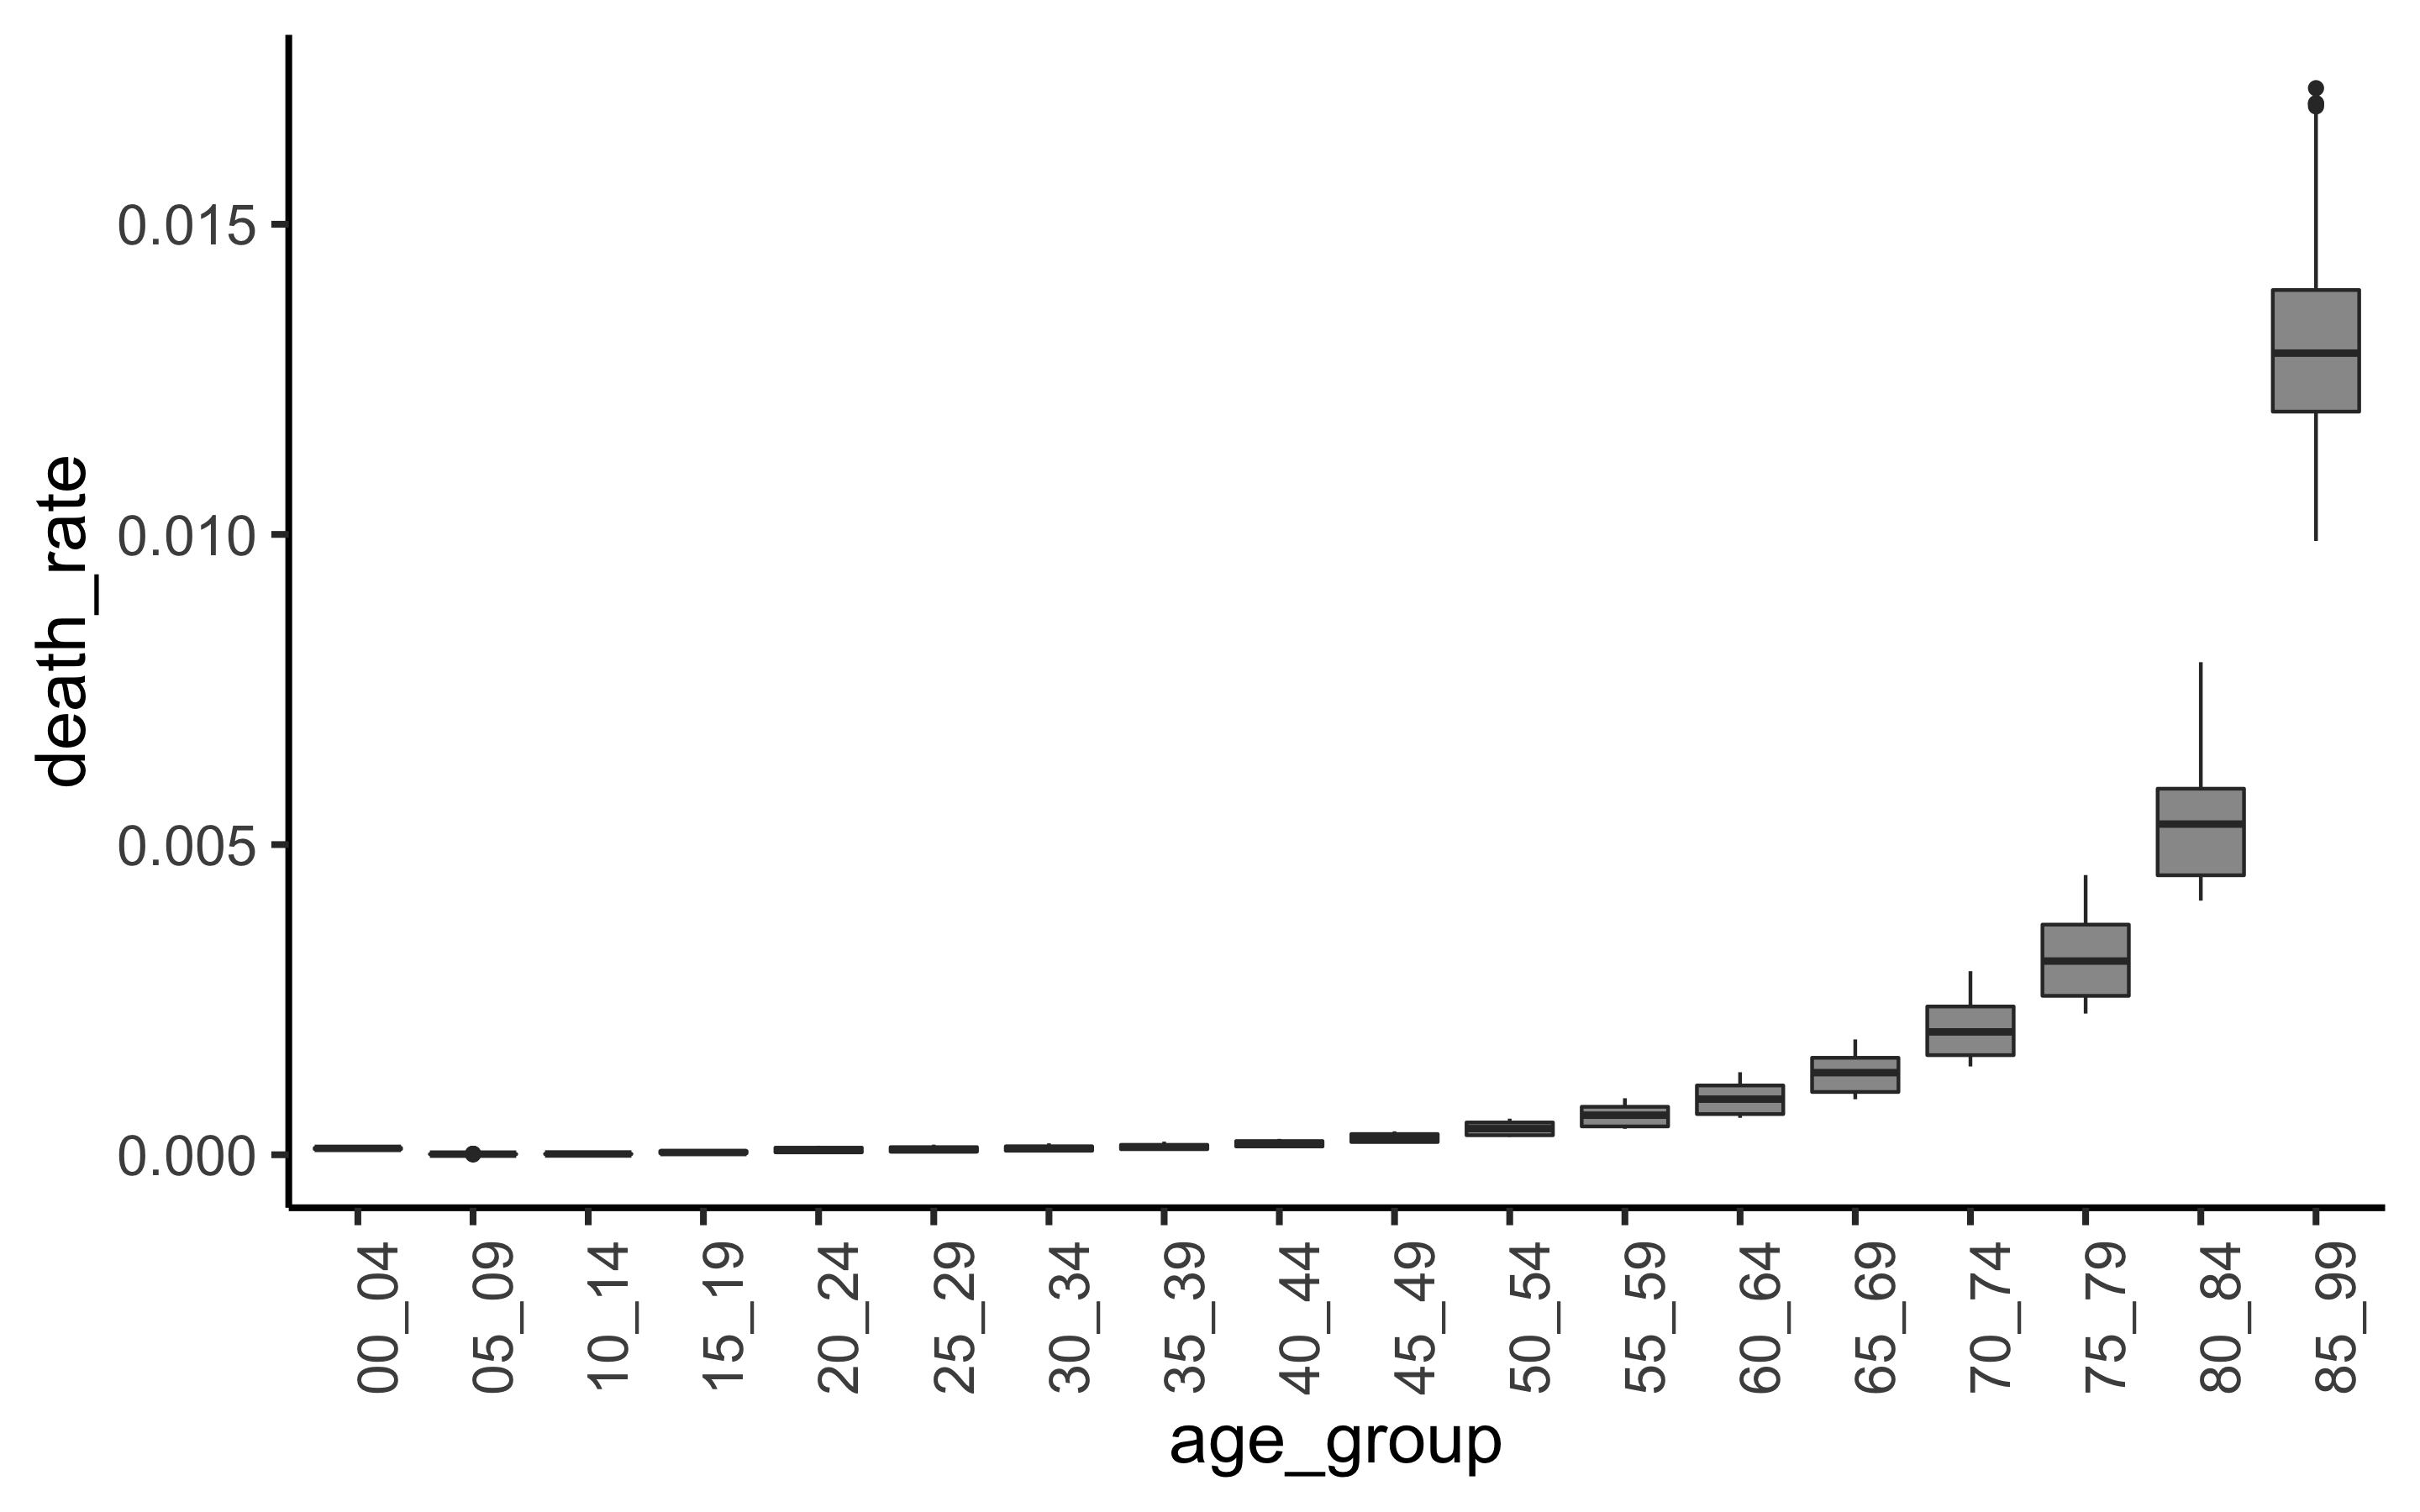
\includegraphics[scale=0.08]{figs/box_plot.png}
\vspace{-2.5mm}
\caption{Box plot of death rate by age group}
\label{fig:box}
\end{wrapfigure}
Looking at the box plot in \cref{fig:box}, we note that death rate increases nonlinearly with age, as the elderly have a significantly higher death rate than all other age groups, and the lowest monthly death rate for the highest age group (85-99) is larger than the highest death rate for the next oldest grouping (80-84).
It appears, unsurprisingly, that age is likely one of the most important factors in determining the death rate for a particular demographic cell. 
\vspace{2mm}

We proceed with an exploratory analysis to examine visual trends in mortality for males and females of different age groups by both month and year (\cref{fig:trends}).
The y-axis in each plot is the death rate (deaths/population) multiplied by 100 (so the numbers can be interpreted as a percent) and the x-axis is either the month (1-January, 2-February, etc.) or year. 
The lines in each plot are the smoothed conditional mean (using the loess method) for the death rate at the specific combination of age group and sex (using the wider bins discussed in \cref{sec:new_vars}) with the gray shading indicating a 95\% confidence interval around the mean\cite{ggplot}.

\begin{figure}
\centering
\begin{subfigure}[t]{0.49\textwidth}
\centering
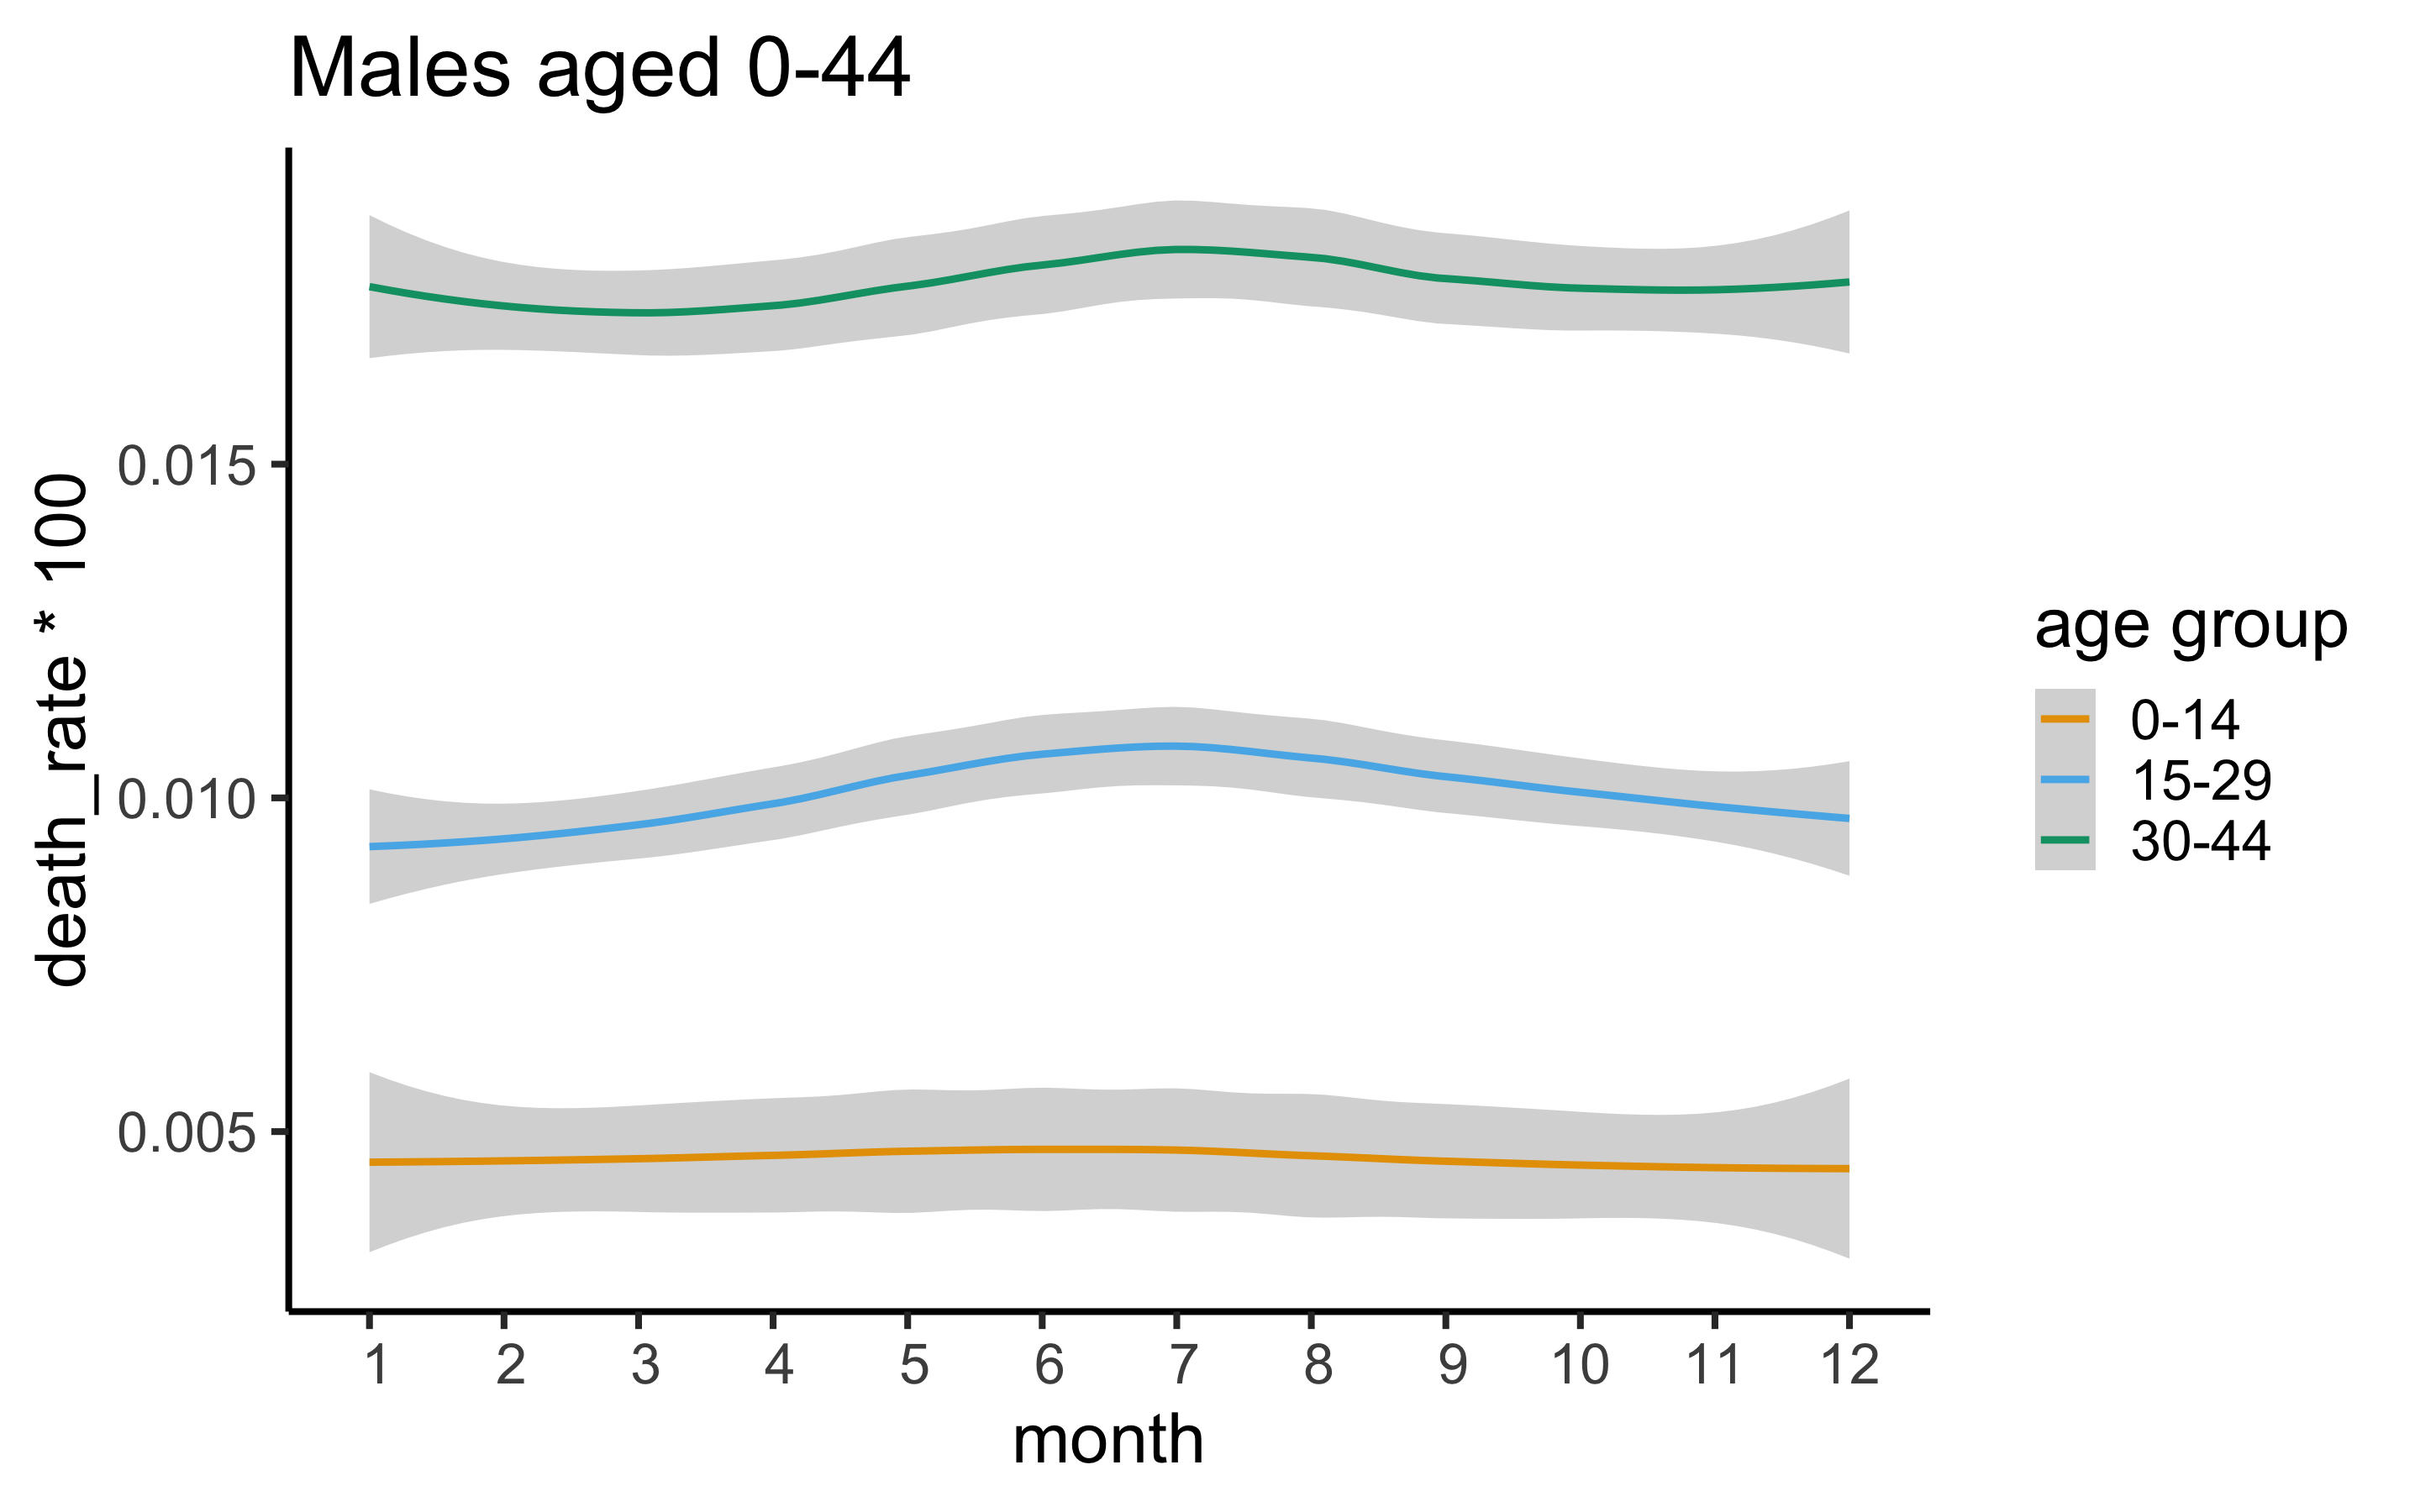
\includegraphics[scale=0.076]{figs/young_men.png}
\caption{Death rate by month for males under 45}
\label{fig:young_men}
\end{subfigure}
\begin{subfigure}[t]{0.49\textwidth}
\centering
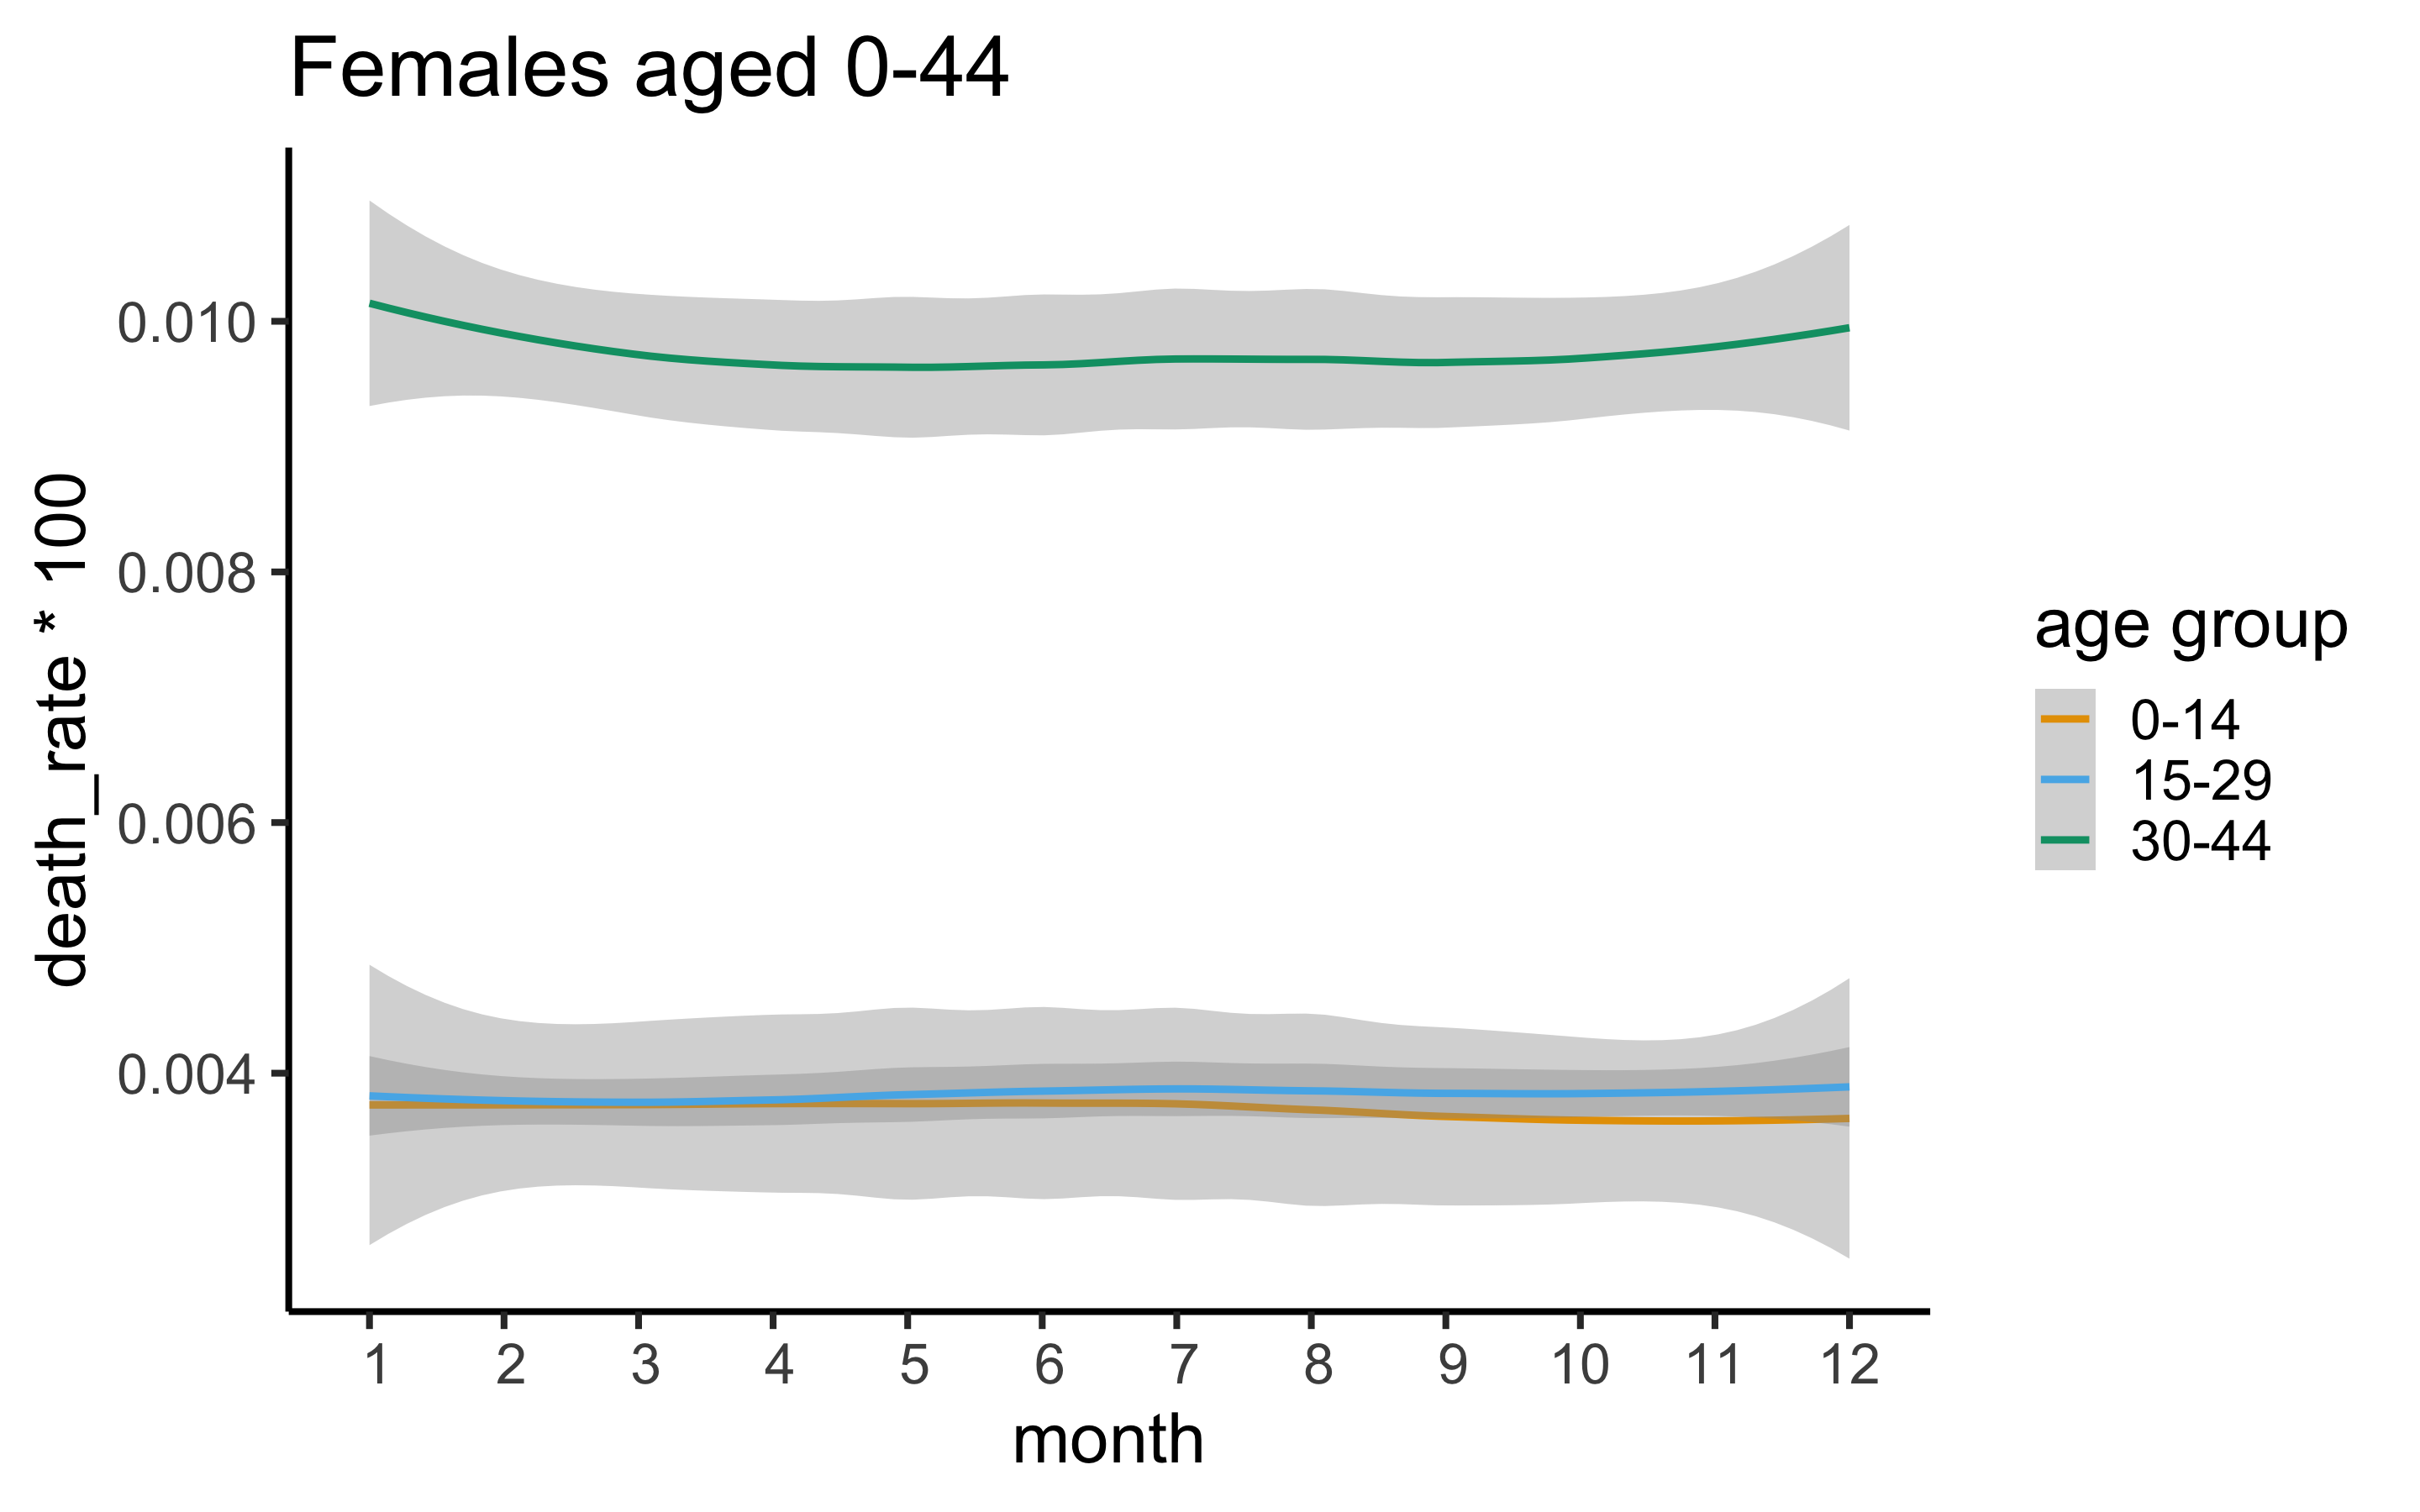
\includegraphics[scale=0.076]{figs/young_women.png}
\caption{Death rate by month for females under 45}
\label{fig:young_women}
\end{subfigure}
\\
\begin{subfigure}[t]{0.49\textwidth}
\centering
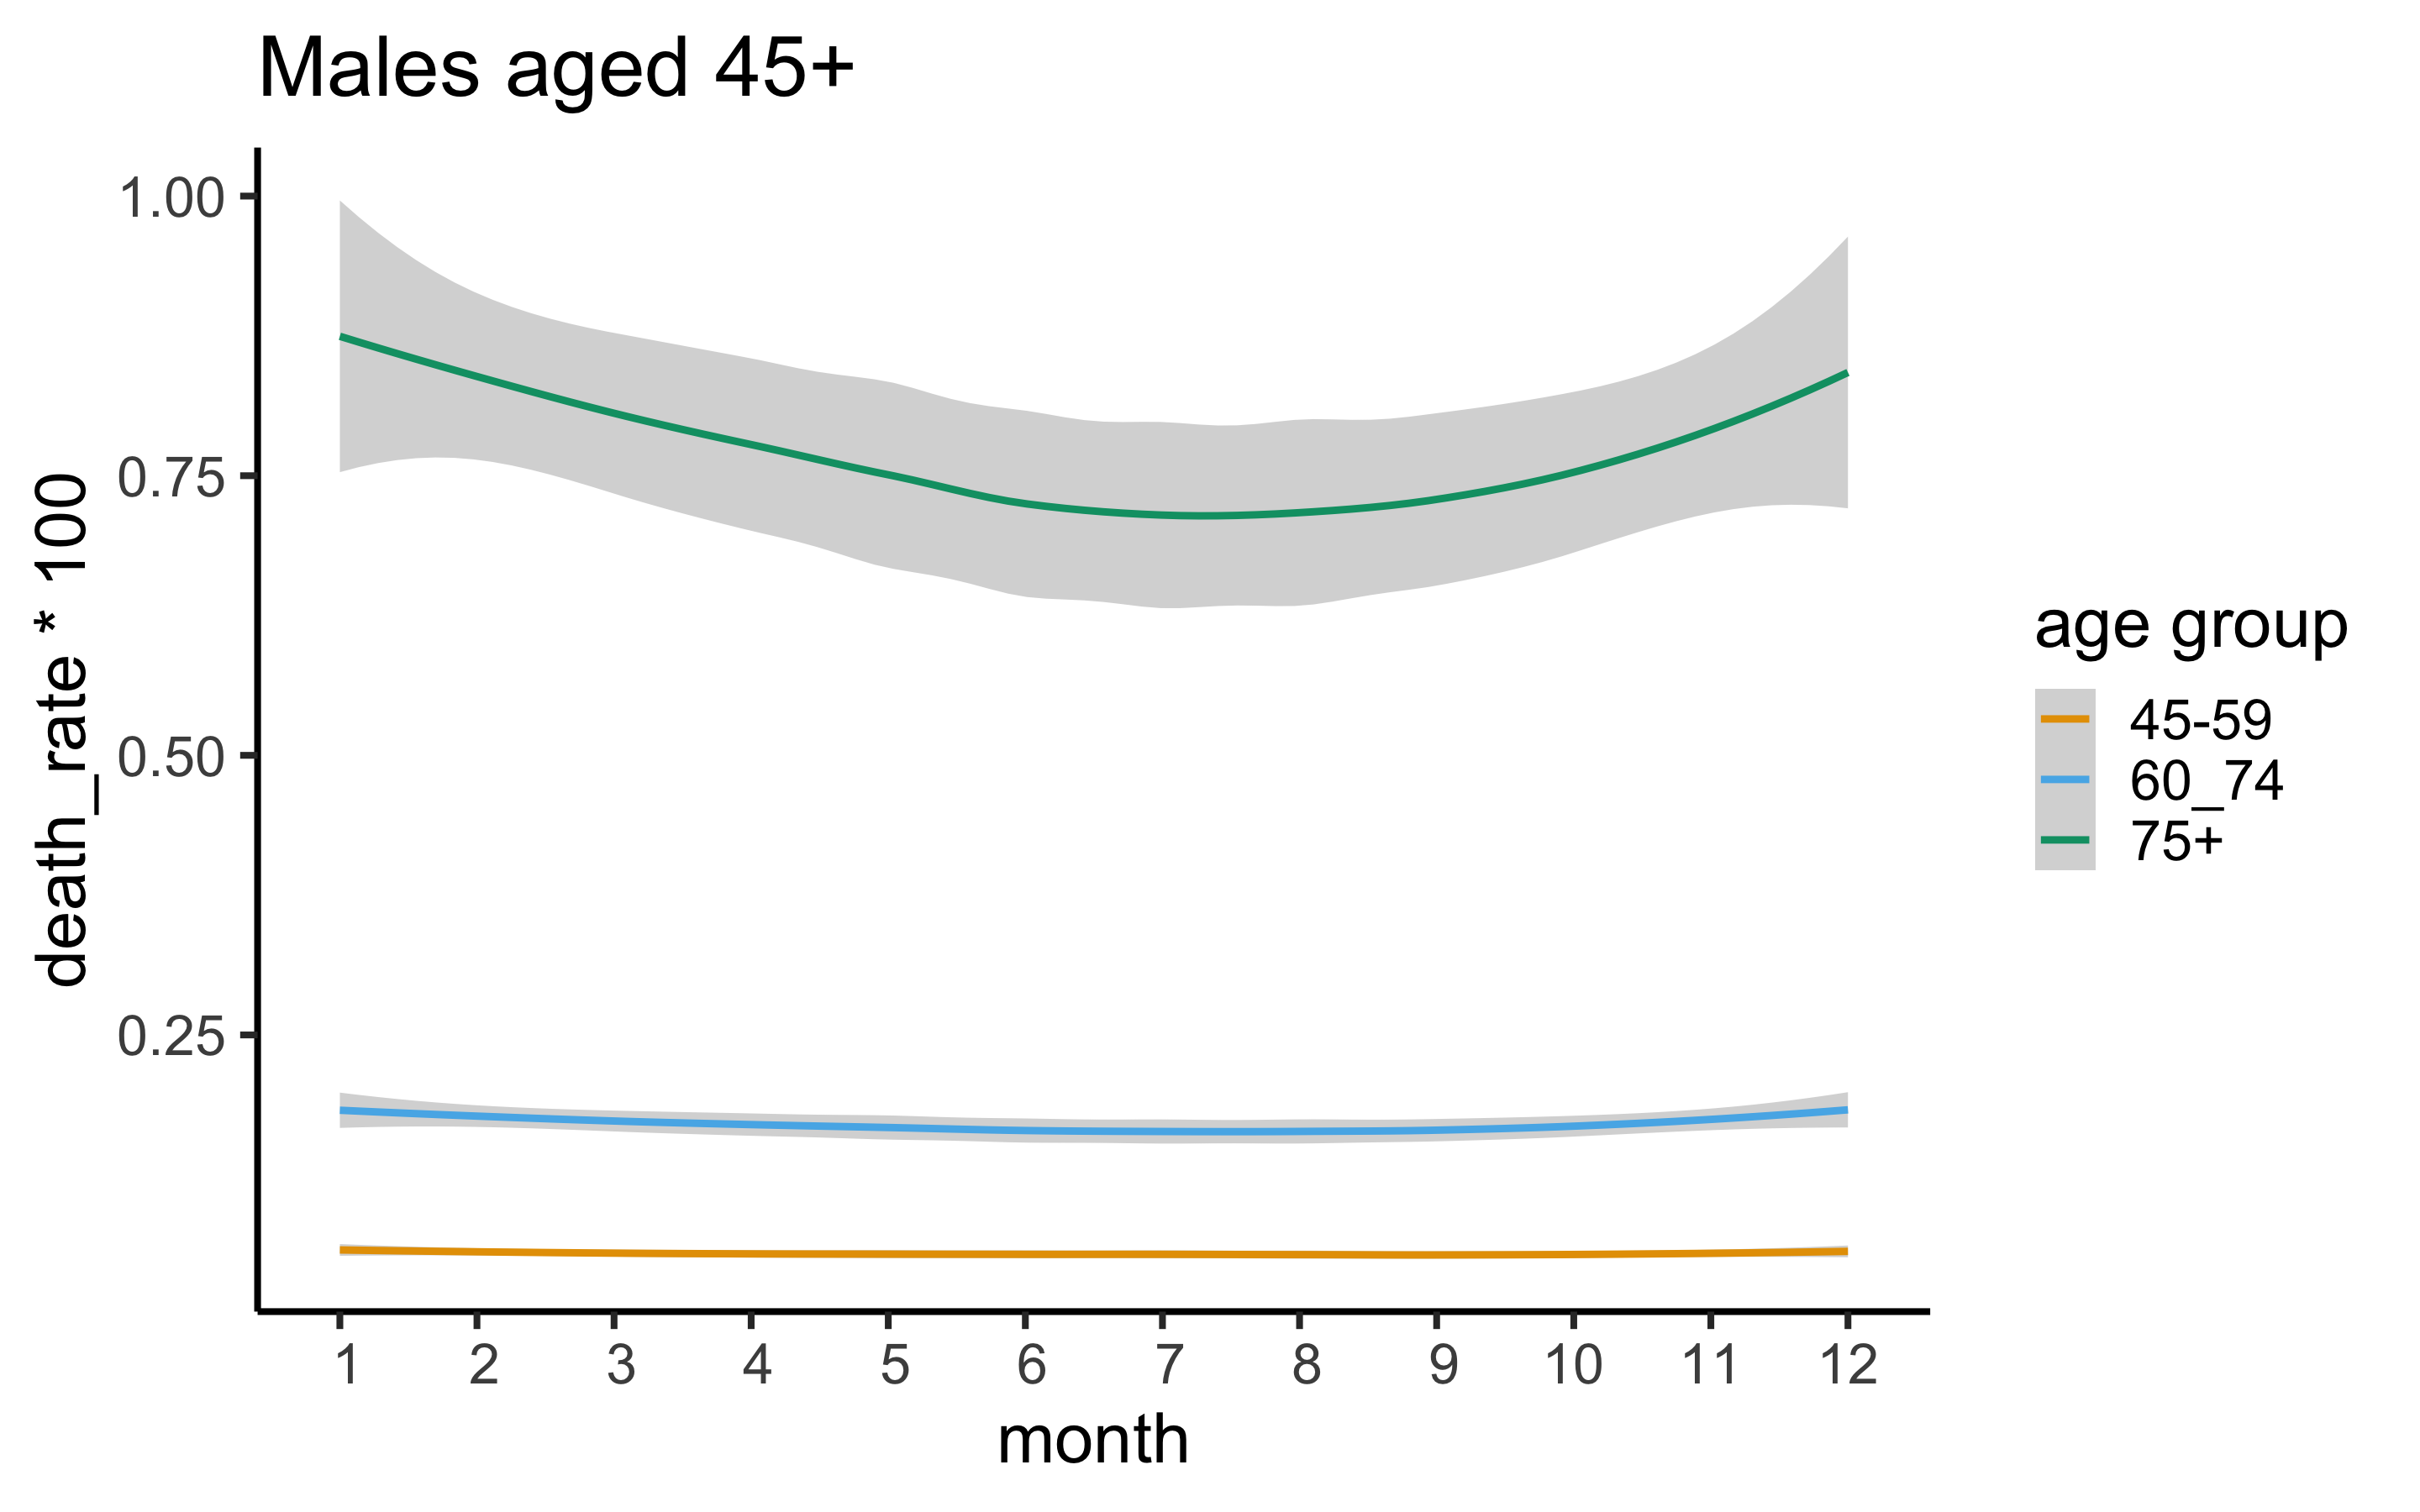
\includegraphics[scale=0.076]{figs/old_men.png}
\caption{Death rate by month for males over 45}
\label{fig:old_men}
\end{subfigure}
\begin{subfigure}[t]{0.49\textwidth}
\centering
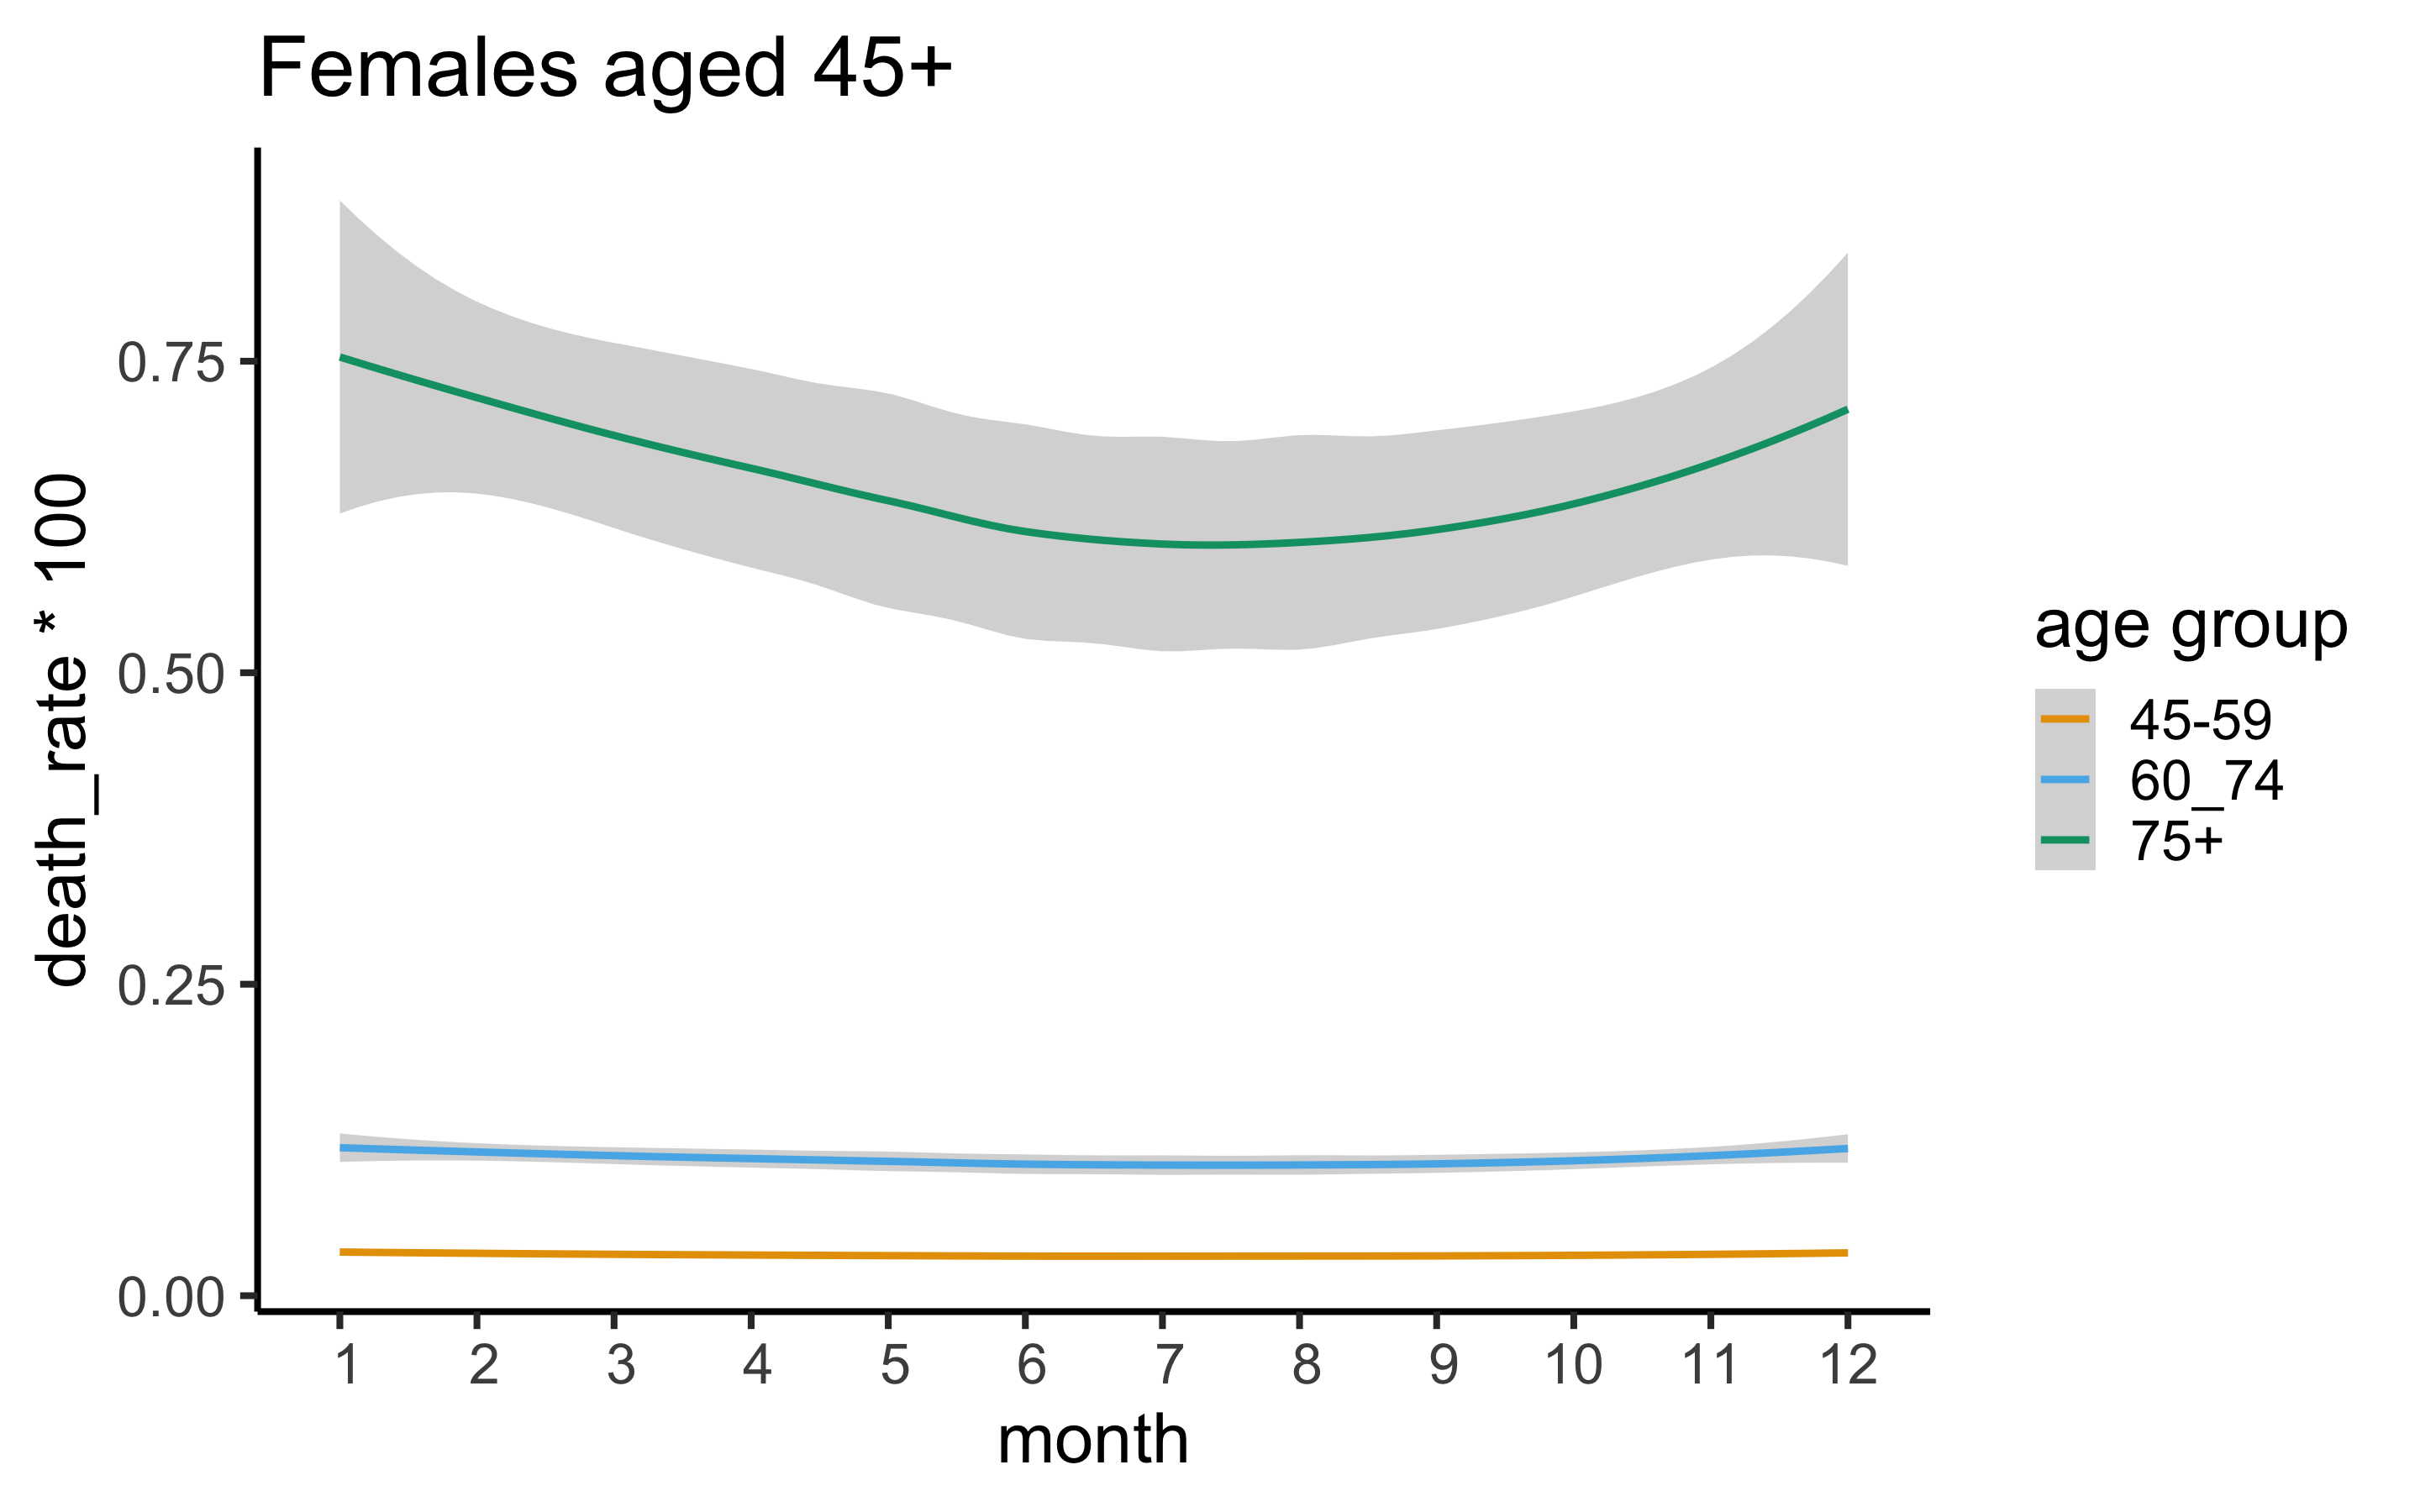
\includegraphics[scale=0.076]{figs/old_women.png}
\caption{Death rate by month for females over 45}
\label{fig:old_women}
\end{subfigure}
\\
%% next set 
\begin{subfigure}[t]{0.49\textwidth}
\centering
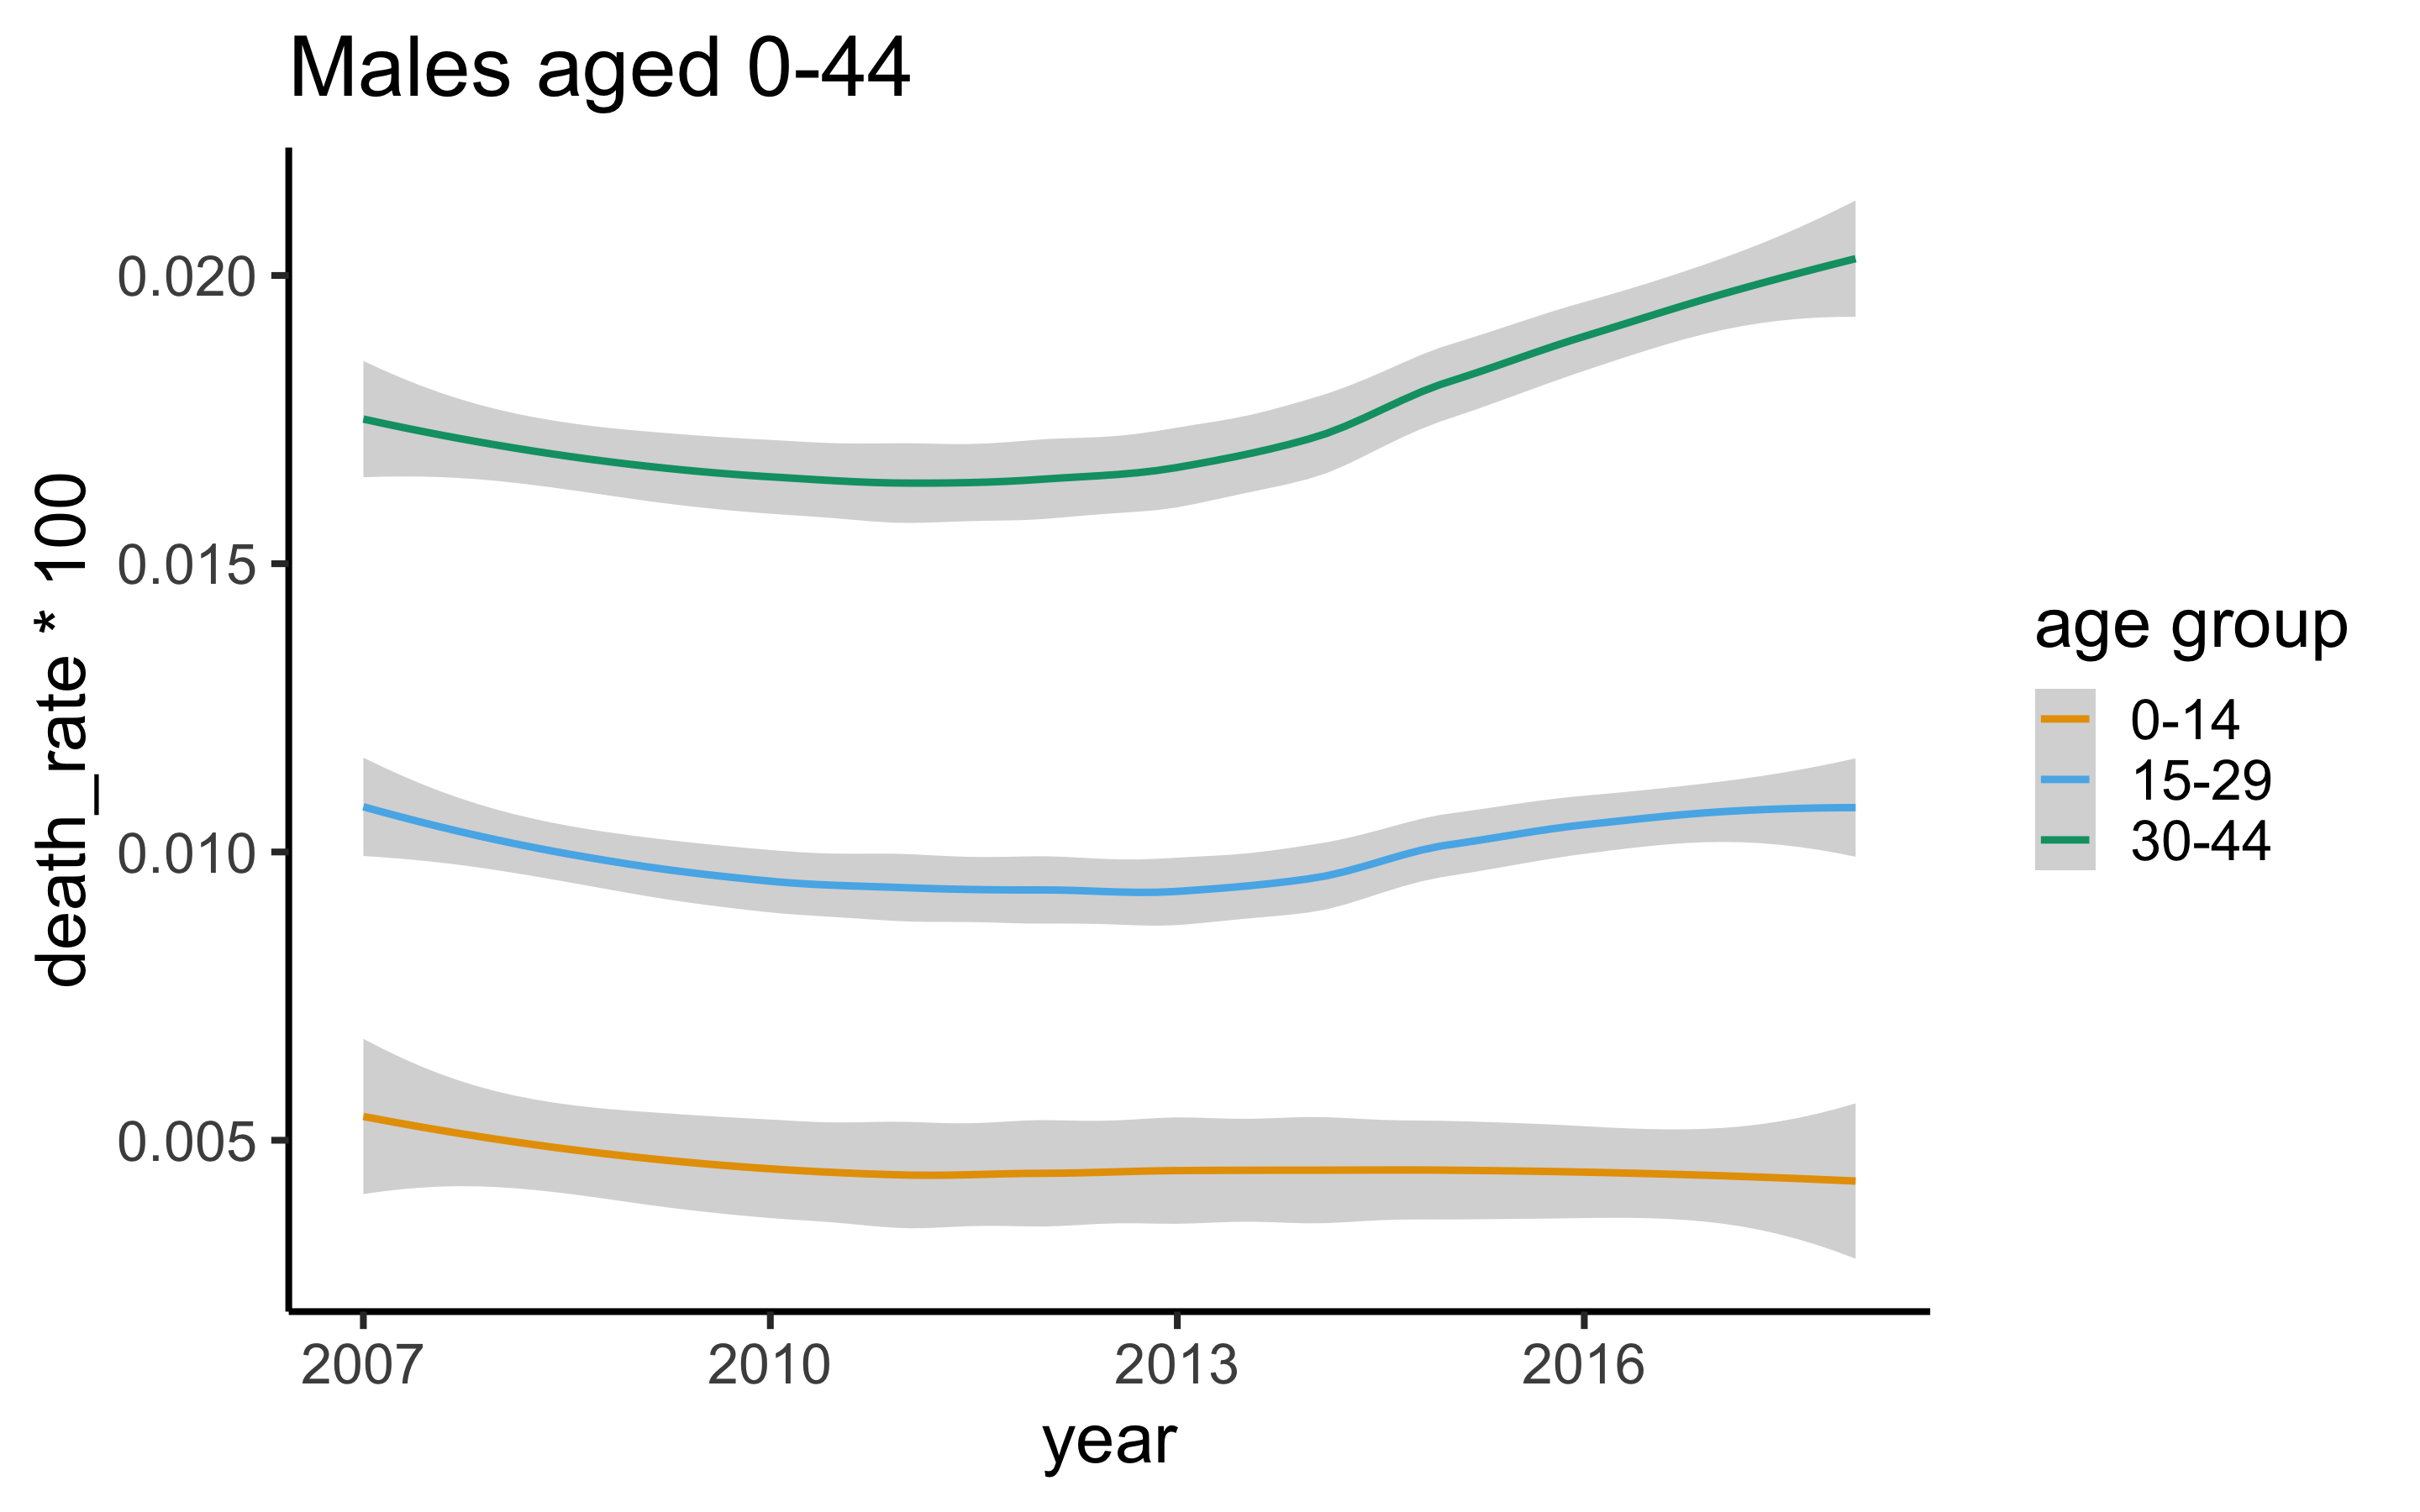
\includegraphics[scale=0.076]{figs/young_men_year.png}
\caption{Death rate by year for males under 45}
\label{fig:young_men_year}
\end{subfigure}
\begin{subfigure}[t]{0.49\textwidth}
\centering
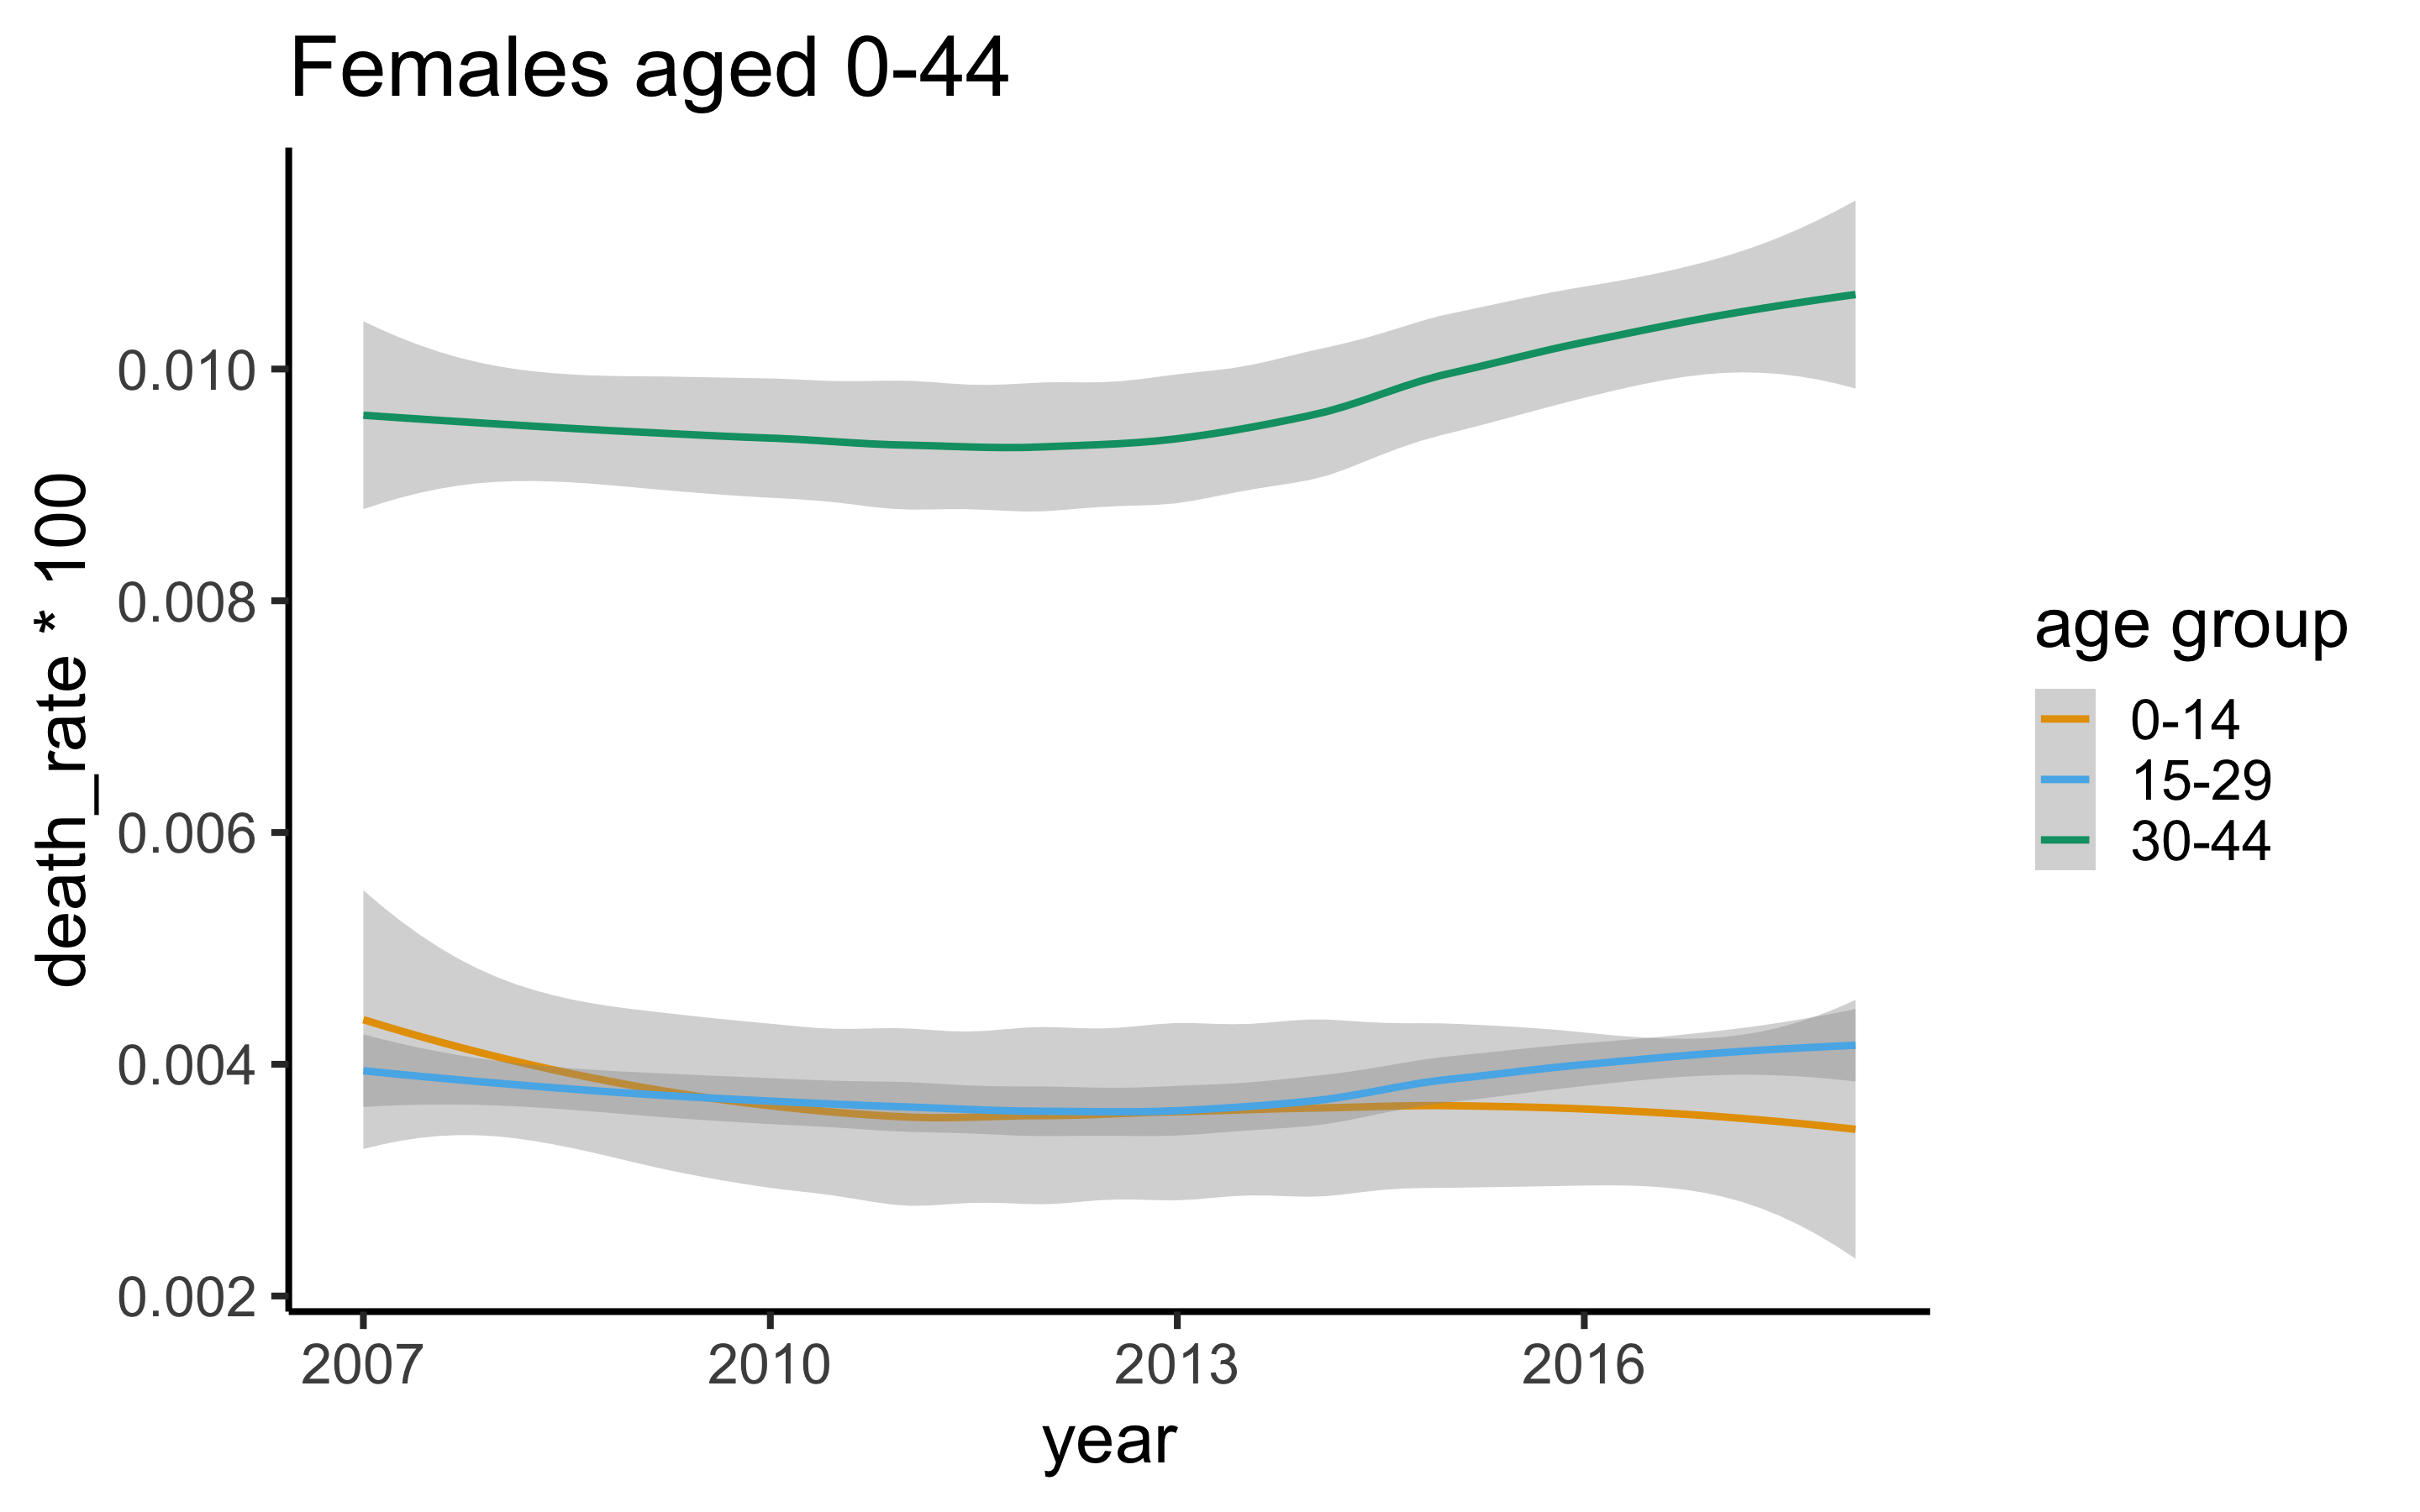
\includegraphics[scale=0.076]{figs/young_women_year.png}
\caption{Death rate by year for females under 45}
\label{fig:young_women_year}
\end{subfigure}
\\
\begin{subfigure}[t]{0.49\textwidth}
\centering
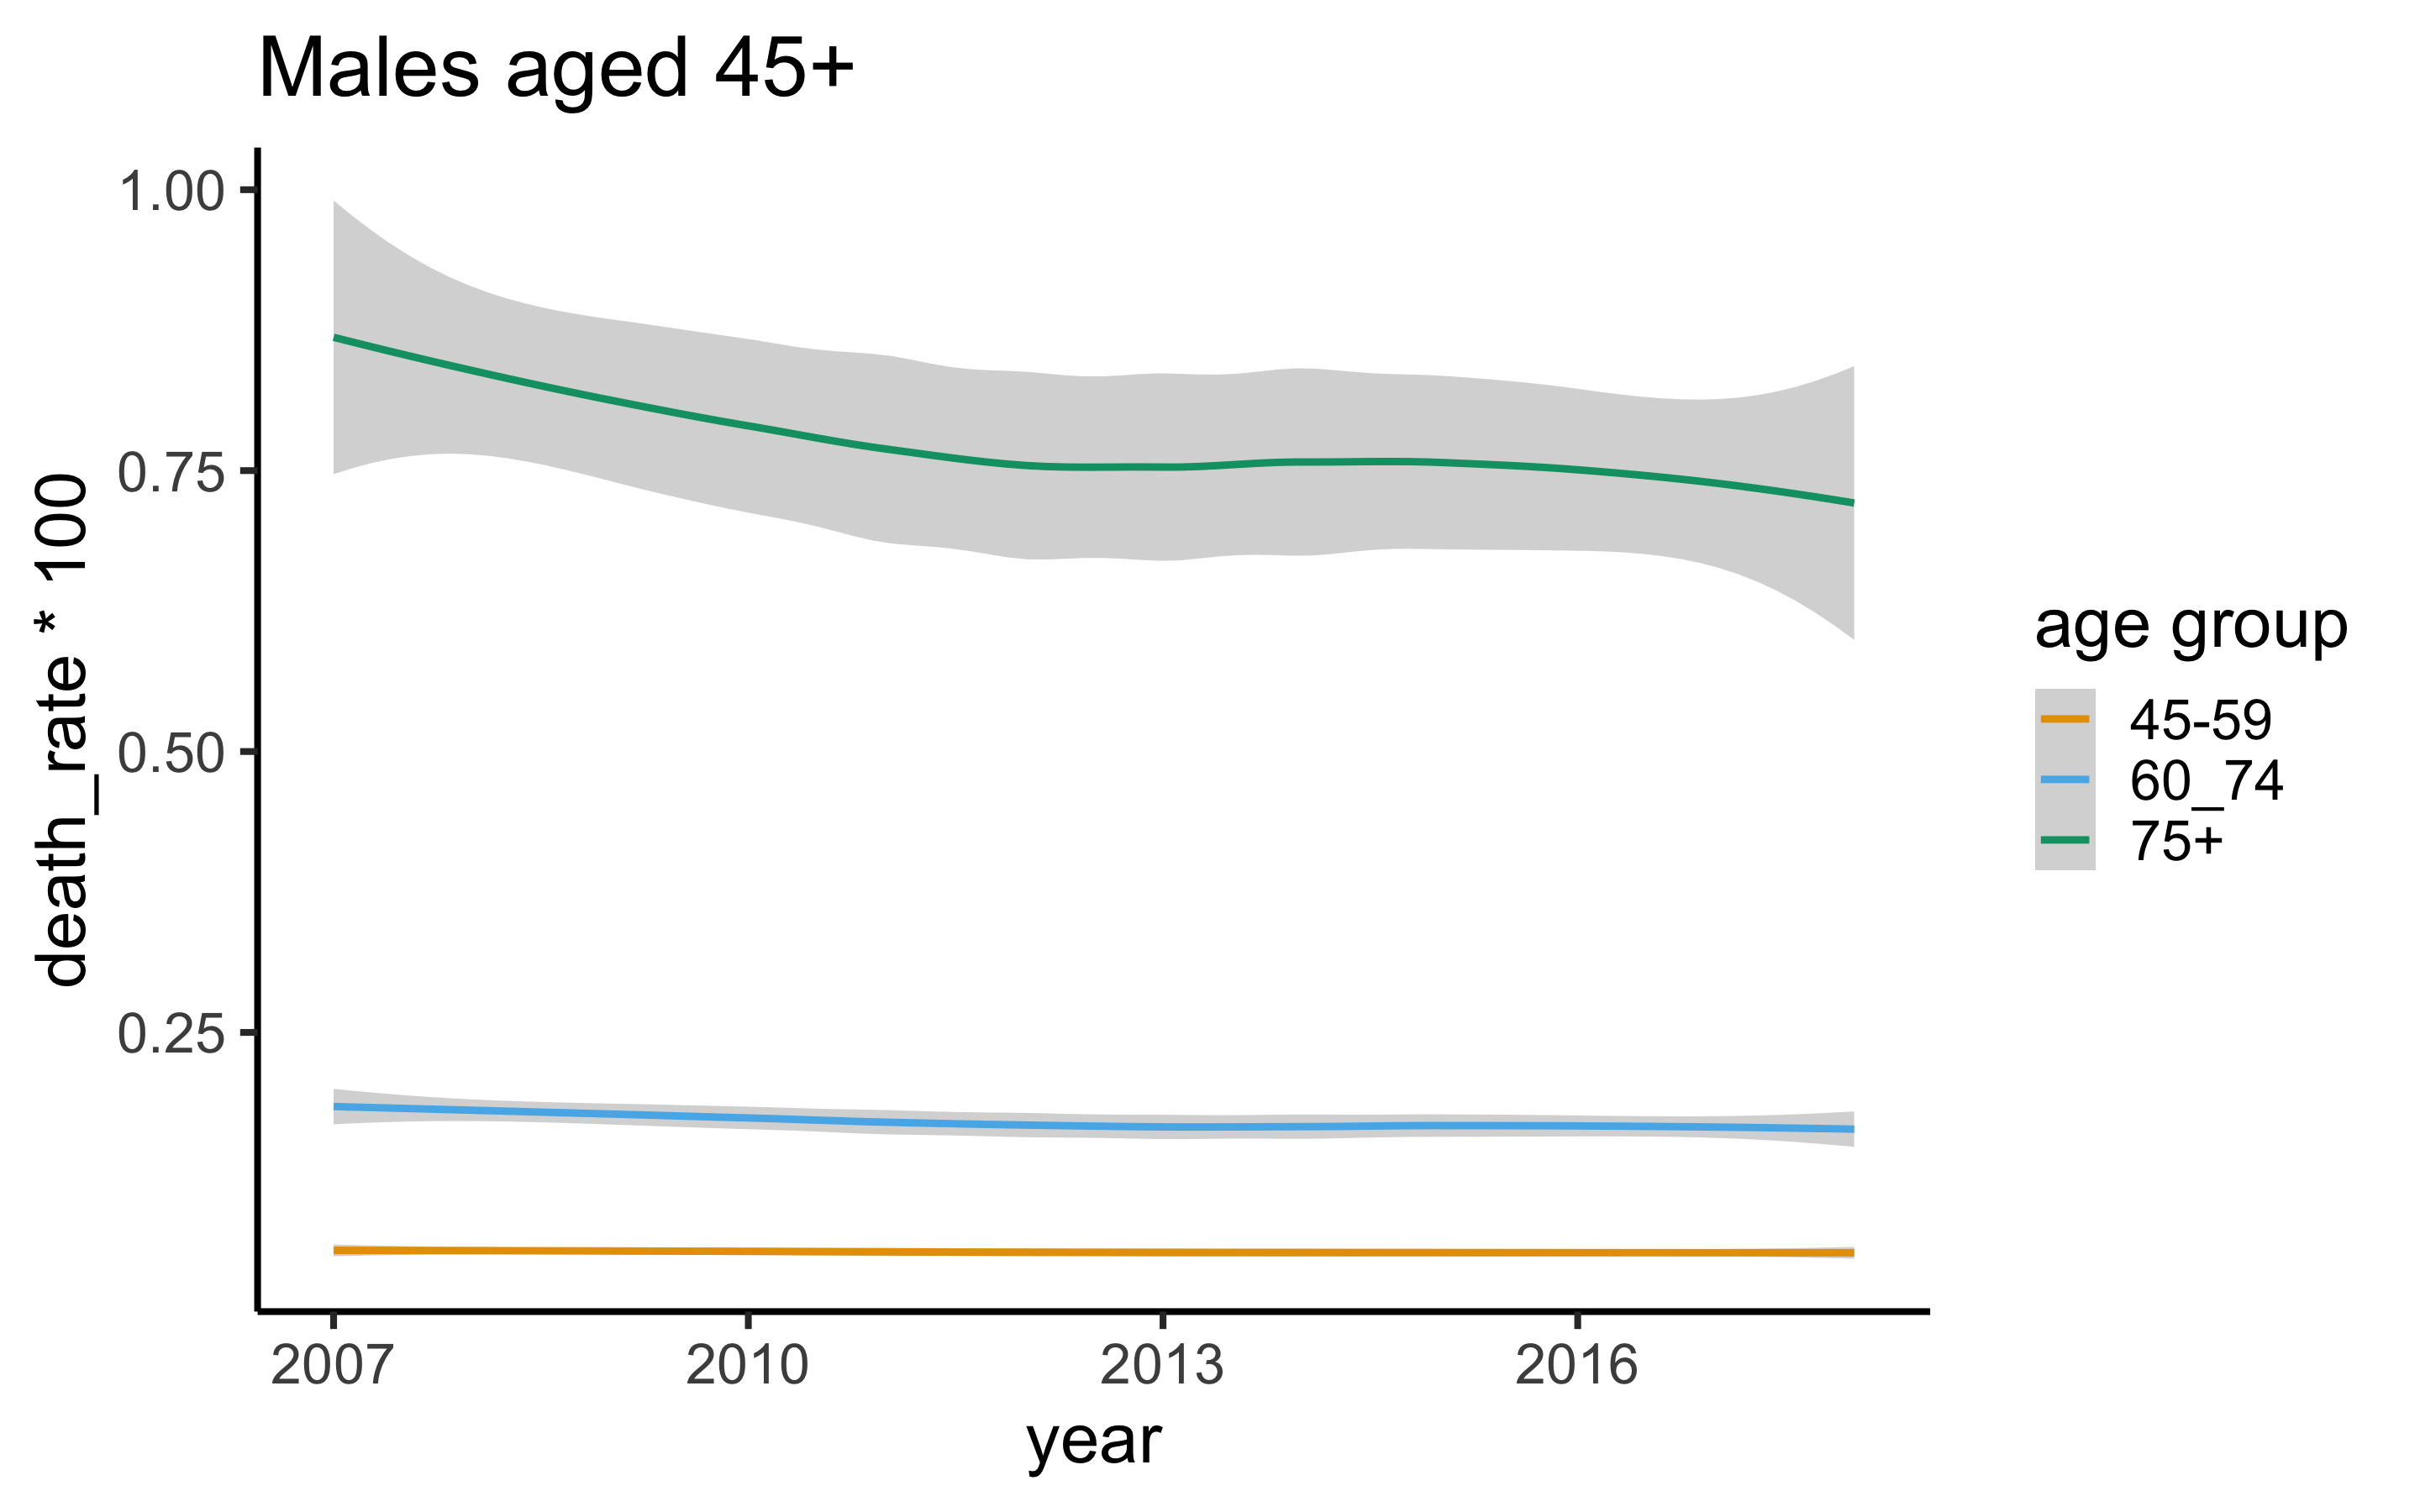
\includegraphics[scale=0.076]{figs/old_men_year.png}
\caption{Death rate by year for males over 45}
\label{fig:old_men_year}
\end{subfigure}
\begin{subfigure}[t]{0.49\textwidth}
\centering
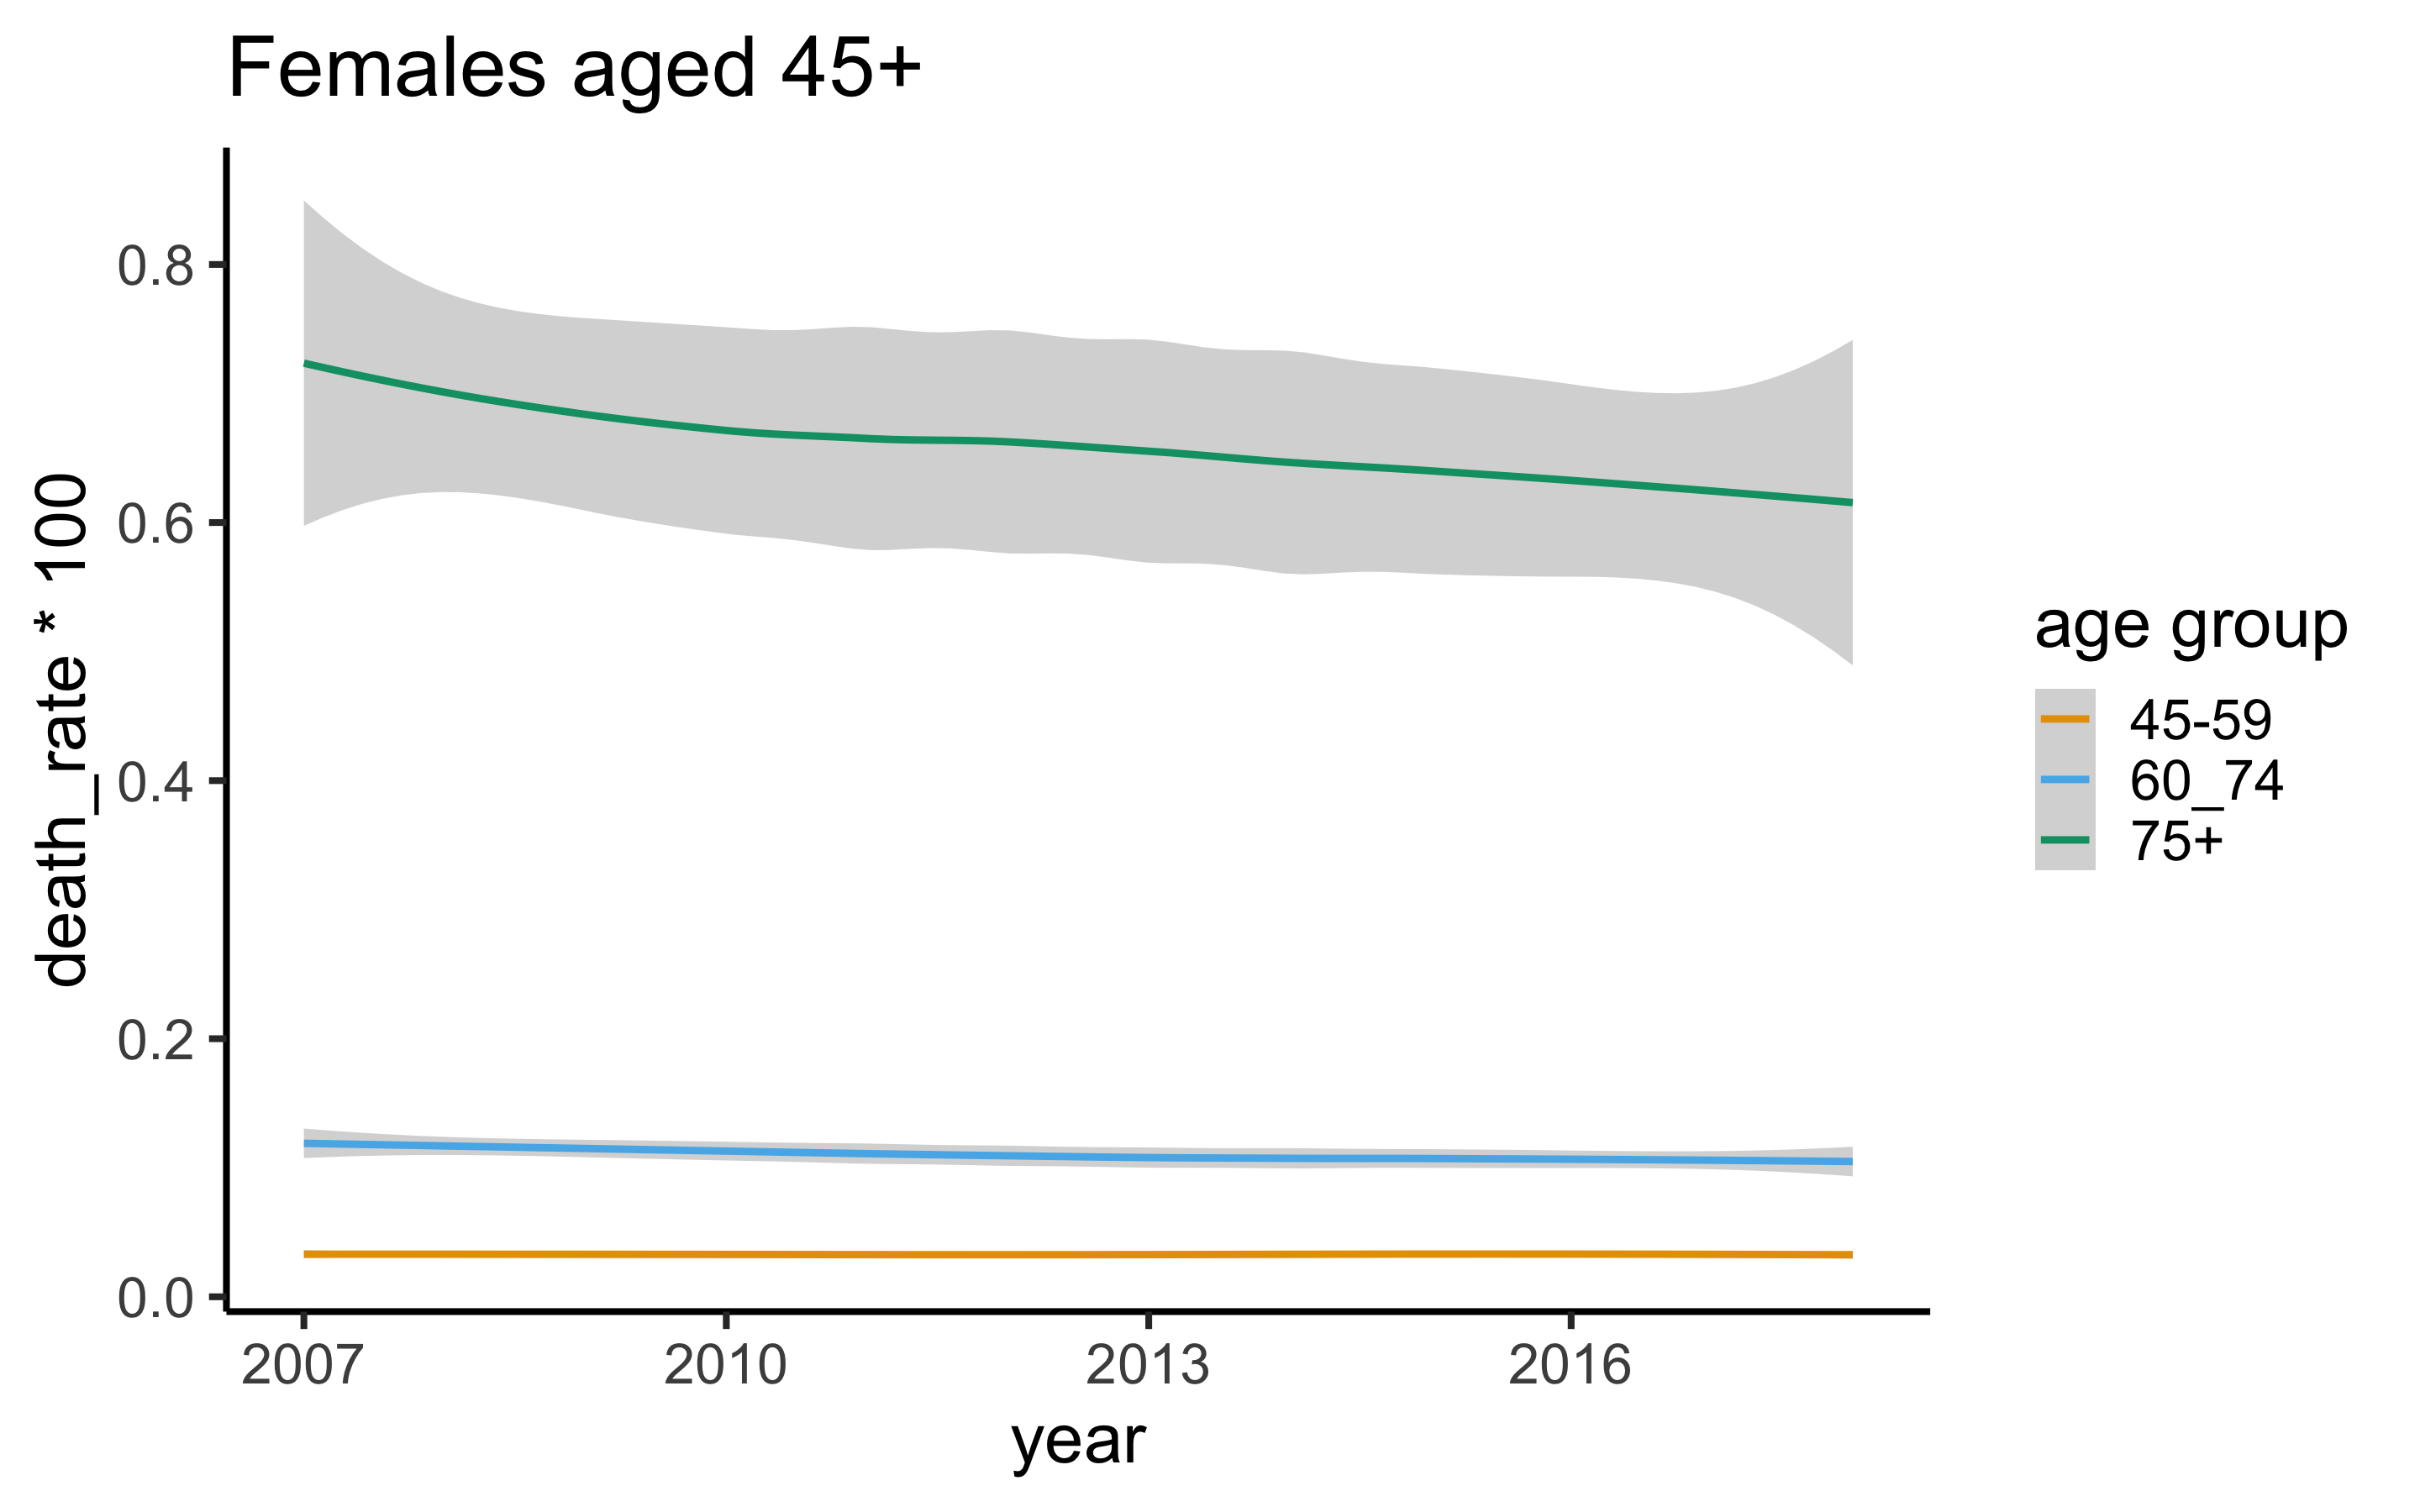
\includegraphics[scale=0.076]{figs/old_women_year.png}
\caption{Death rate by year for females over 45}
\label{fig:old_women_year}
\end{subfigure}
\caption{Seasonal and year-over-year trends in death rate broken down by age and sex}
\label{fig:trends}
\end{figure}


\subsection{Analyzing seasonal variation by age and sex}\label{sec:age_sex}

We first direct the reader's attention to an interesting trend in \cref{fig:young_men} and \cref{fig:young_women}.
At the 0-14 age group, it seems that males and females have approximately the same death rate, approximately 0.004\%, and the rate is, for all intents and purposes, the same in each month. 
At the 15-29 and 30-44 age groups, however, not only do males have a noticeably higher average death rate, approximately 2x the female rate in the 15-29 age group and rougly 1.7x the female rate in the 30-44 age group, but there also appears to be a rise in male deaths in the summer months that is not necessarily apparent in the summer months for females.
There is another apparent seasonal trend as \cref{fig:old_men} and \cref{fig:old_women} indicate increased death rates for seniors (75 and over) in the winter months, likely due to seasonal illnesses such as influenza and pneumonia.

\subsection{Year-over-year mortality trends}\label{sec:age_year}

Another trend that is visible in the graphs concerns the decline and rise in death rates among different age groups across the years in our sample.
In \cref{fig:young_men_year} and \cref{fig:young_women_year}, there appears to be an increase in the death rate in the 30-44 age group, among both men and women, particularly since 2013.
Further research could be done on more specific data (i.e., broken down by geography or race) to try to identify potential causes, but for the purposes of this report it suffices to note the trend and think about strategies for modeling it in later analyses.
One positive trend in the data is in \cref{fig:old_men_year} and \cref{fig:old_women_year}, where the 75 and over age group appears to have a linearly declining death rate over the last 12 years (possibly due to advancements in treating cancers and other diseases that affect the elderly).
Notably, both of these trends appear to be consistent between males and females, though men still tend to have higher mortality rates than women in general.


\section{Modeling Death Rates with Generalized Linear Models}\label{sec:glms}

Since the goal of our analysis is to come up with a model for the count of the number of deaths, a generalized linear model with Poisson distribution and log link function would likely be the most appropriate.
This approach is common in existing research around mortality, as in \cite{strumpf2017}.
Since the total population for each combination of year, age group, and sex is different, we'll want to account for this in our model, as a way to look at death \textit{rates}, rather than raw counts.
As a result, we'll use the log of the population as an offset term in all GLMs that we fit\cite{agresti_2019}.

\subsection{Poisson regression}\label{sec:poisson}

We considered three different Poisson regression models with both the original age bins and the wider age bins and then compared the models using AIC and BIC (shown in \cref{tab:ICs}) to choose the age bins we would use in further analyses. 
The first model, \textbf{model 1}, can be considered as a base model--it only includes main effects for each of the variables \verb+age+, \verb+sex+, \verb+year+, \verb+summer+, and \verb+winter+, where \verb+age+ represents whichever age bin is being used (wide or original). 
\textbf{Model 2} introduces pairwise interactions between the \verb+age+ variable and both the \verb+winter+ and \verb+summer+ variables, as well as the \verb+year+ variable, to account for the higher death rate among elderly people in winter months, possible increased deaths among the young in the summer, and the differing trends in mortality over the last 12 years between older people and middle aged people discussed in \cref{sec:age_year}.
Finally, \textbf{model 3} maintains the pairwise interactions of \textbf{model 2}, but instead of using indicators for summer and winter, instead uses indicator variables for each month, to model trends in the relationship between the month and the death counts that don't fall neatly into the summer/winter/other grouping scheme.

% latex table generated in R 3.6.2 by xtable 1.8-4 package
% Thu May 14 19:37:11 2020
\begin{table}[ht]
\centering
\begin{tabular}{lrrr}
  \hline
Model & AIC & BIC & Test Set MSE \\ 
  \hline
model\_1\_wide & 5582868 & 5582930 & 0.3961 \\ 
  model\_2\_wide & 5565020 & 5565173 & 0.3938 \\ 
  model\_3\_wide & 5483852 & 5484338 & 0.3950 \\ 
  model\_1\_original & 311842 & 311977 & 0.0362 \\ 
  model\_2\_original & 281677 & 282126 & 0.0316 \\ 
  model\_3\_original & 247811 & 249255 & 0.0306 \\ 
   \hline
\end{tabular}
\caption{AIC, BIC, and MSE for poisson regression models} 
\label{tab:ICs}
\end{table}


\subsection{Model selection via AIC and MSE}\label{sec:aic}

For both age groupings (the original groups in the data and the wider bins discussed in \cref{sec:new_vars}), model 3 has the lowest AIC and BIC, followed by model 2 then model 1. 
Since a lower information criteria is preferable, this gives support to choosing model 3 and using the original (narrower) age groupings.
Since AIC and BIC penalize model complexity (with the penalty for number of model parameters scaling with the sample size in BIC), it is notable that the lowest AIC and BIC correspond to the most complex model, model 3.
And yet, while model 2 does slightly better than model 1 (a much simpler model), model 3 presents a more substantial improvement over model 2, even though it has even more parameters (due the change from modeling seasonality in three bins to twelve bins).

We also can calculate the mean squared error (on the log scale) for prediction for each of the models (using the same 2/3 train 1/3 test split as in \cref{sec:ml}). 
These results are presented in \cref{tab:ICs} and generally comport with the results from the information criteria calculations.
The narrower age bins models do a much better job in predicting death counts for held-out data than the coarser bins models do, as evidenced by the significantly lower MSE.
Within each age binning scheme, however, the MSEs are not substantially differenct, though models 2 and 3 do show a slight improvement over model 1, which could reflect the importance of the interaction terms in explaining variation in mortality. 

\subsection{Using a quasipoisson model to correct for possible overdispersion}\label{sec:qp}

Though Poisson regression is commonly used for count data, it may be inappropriate if the mean-variance relationship does not hold.
When the variance is greater than the mean, a phenomenon known as overdispersion, it may instead be appropriate to use quasipoisson regression, which allows the variance to be equal to some constant times the mean, rather than just the mean\cite{agresti_2019}. 
We fit each of models 1, 2 and 3 using quasipoisson regression instead of Poisson regression and retrieved the estimates for the dispersion parameter to see if we needed to account for overdispersion in our models. 
In each of the models, we get a large value for the dispersion parameter (in the range of 60-80), indicating that the data may not follow a Poisson distribution. 

AIC is not defined for quasi-families, so we'll again compare our models using a test set MSE.
The results are the same as those in \cref{sec:aic}, with models 1 and 3 reporting a test set MSE of 0.0362 and 0.0306, respectively, and model 2 with a test set MSE of 0.0316. 
The overdispersion for which we are correcting is connected to the variance parameter being estimated, however, so it mainly affects the inference (i.e., length of confidence intervals), and we'll want to use the quasipoisson models to report any trends we find in the data.

\subsection{Detecting trends in mortality from regression coefficients}\label{sec:inference}

To look at how mortality has changed by year for different age groups, we can compute the average slope on \verb+year+ in each age group as estimated by the quasipoisson model\cite{emmeans}.
\Cref{fig:em_plot} shows these estimated slopes with error bars mapping the 95\% confidence interval for the slope estimate. 
Notably, all age groups 65 and older have seen improvements in death rates since 2008 (in the form of a negative \verb+year+ slope) and the confidence intervals for these slopes exclude 0, indicating a statistically significant result. 
Another notable trend is the positive estimated slope for \verb+year+ in the 25-39 age groups, all with confidence intervals excluding zero.
The year trend is the log of the risk ratio, so for the 35-39 age cohort, we would expect on average the death rate to increase by around $\exp(0.03) \approx 1.03$ times each year.
These estimates concur with our observations in \cref{sec:age_year}, highlighting a worrying trend of increasing death rates for younger and early middle-aged adults.
One positive trend (which was not apparent in \cref{fig:trends}) is that the youngest age group (0-4 years) also has a statistically significant downward trend, indicating a decline in child mortality.

\begin{figure}
\centering
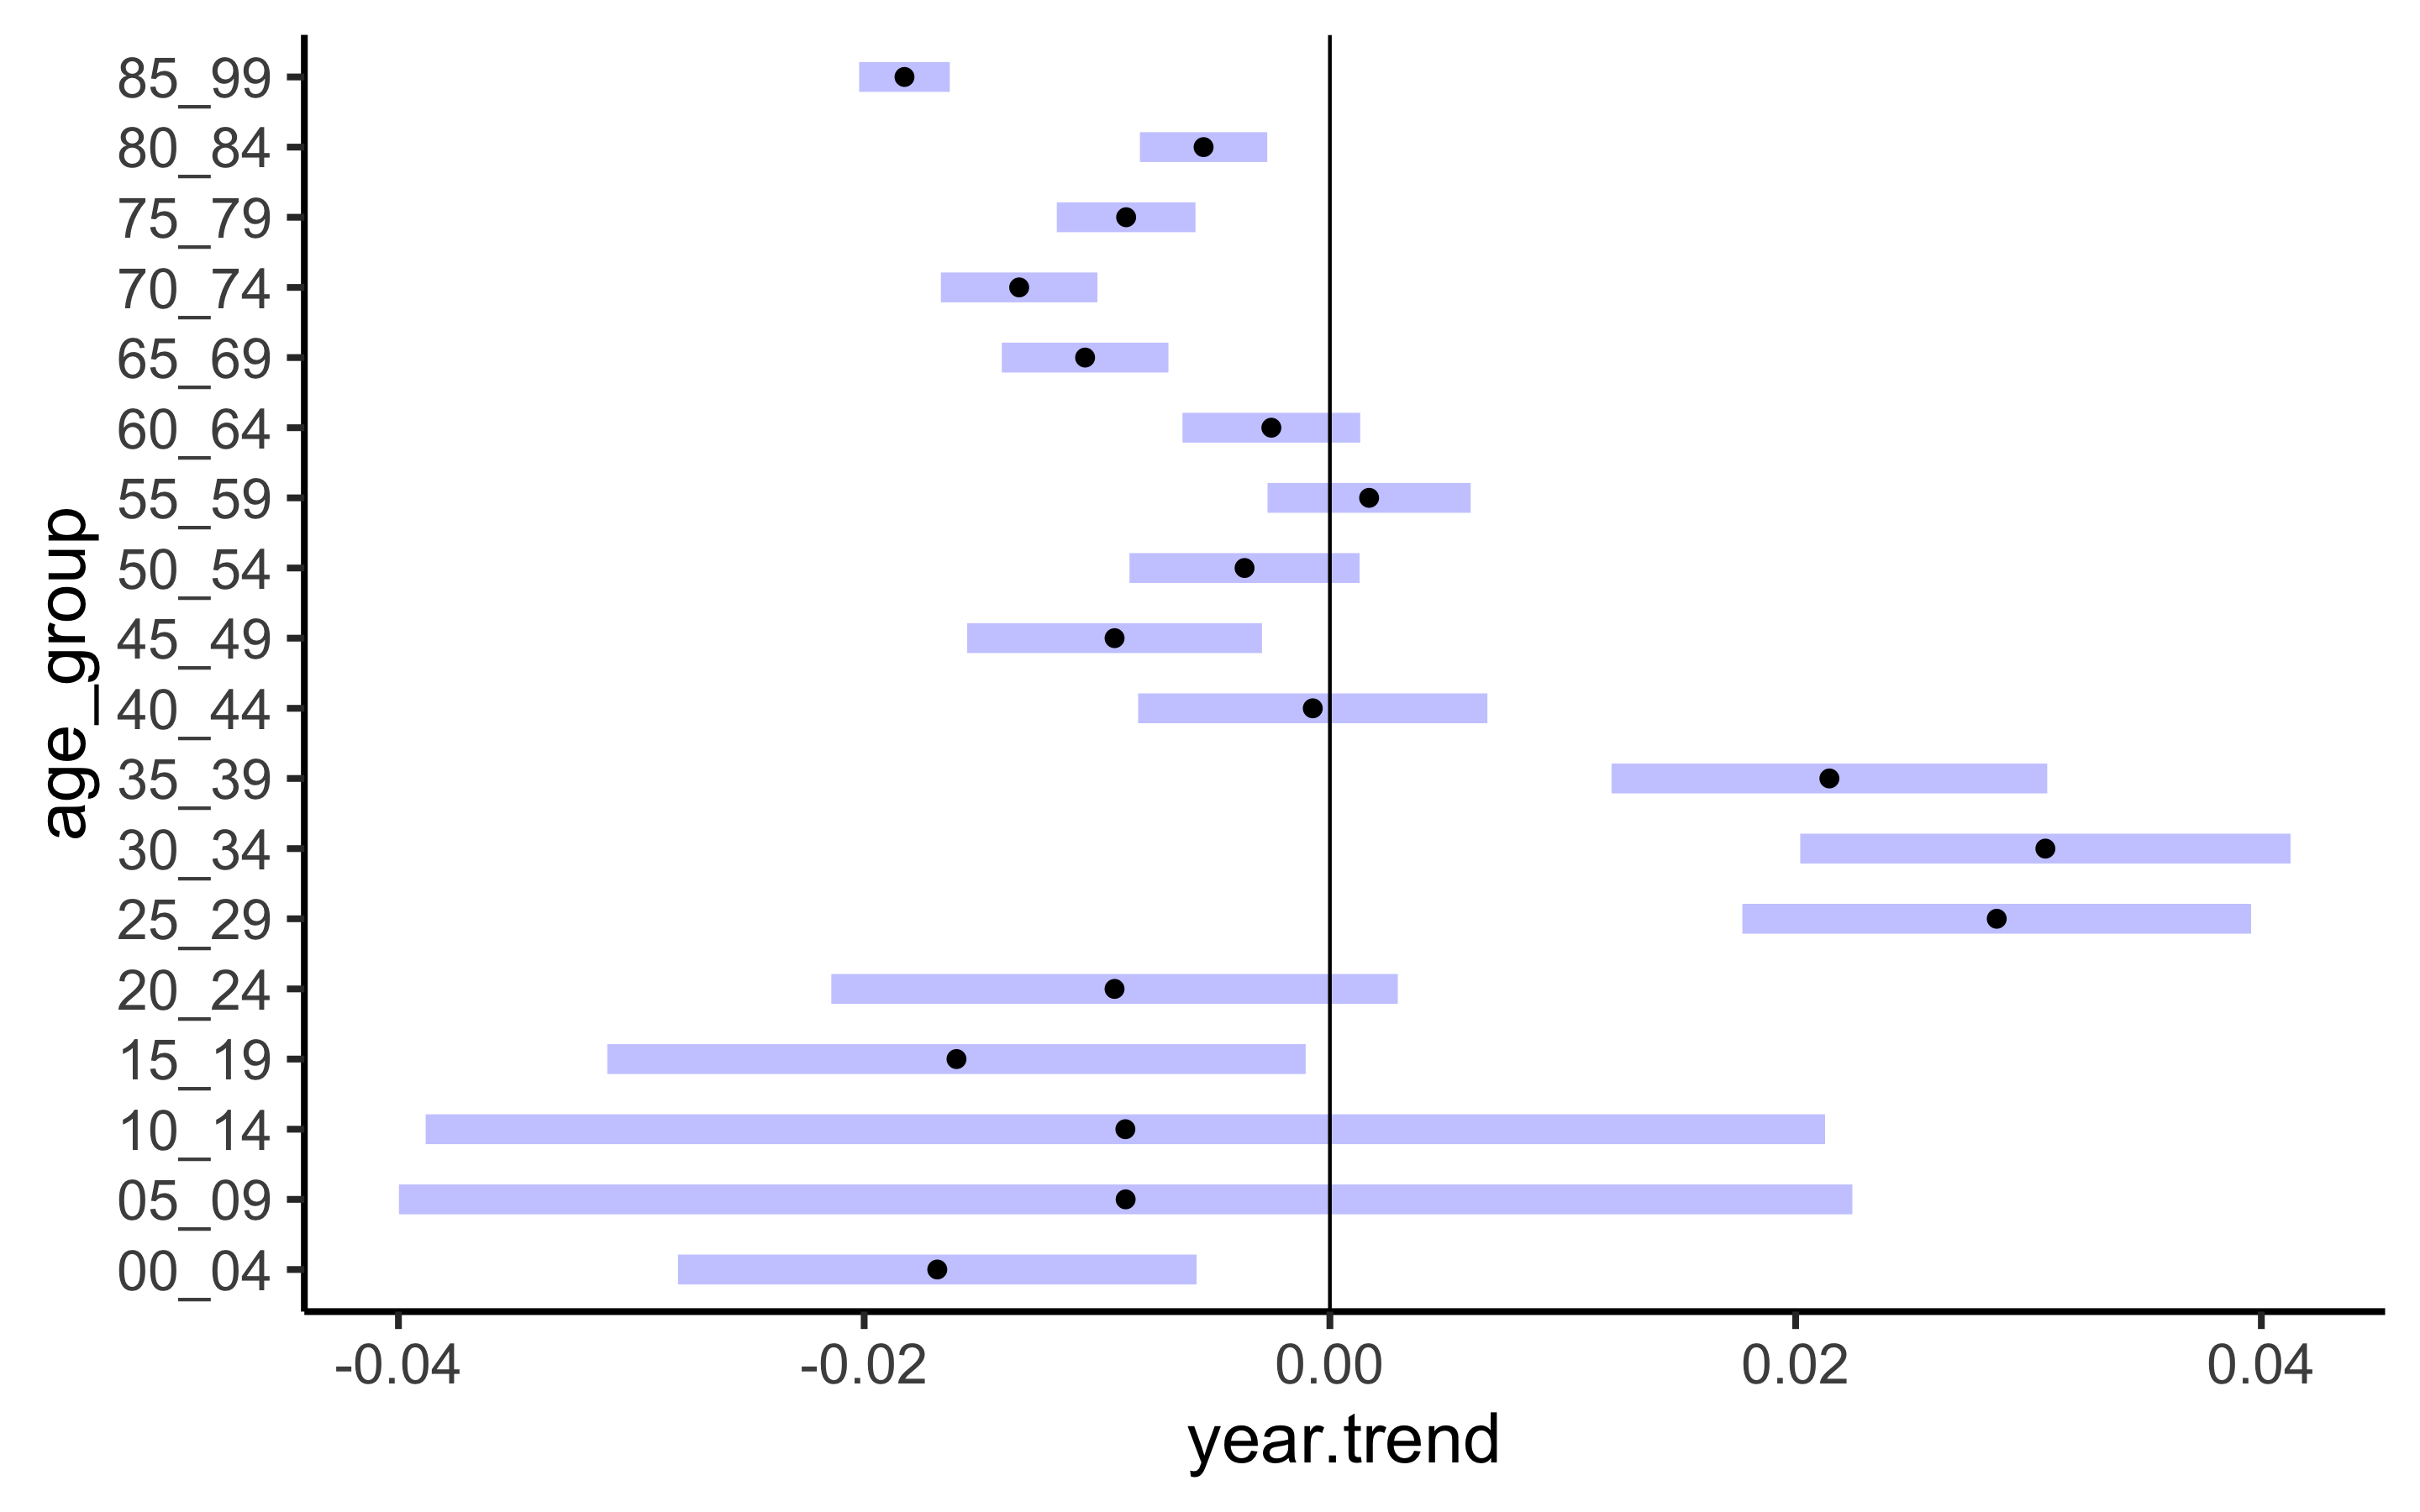
\includegraphics[scale=0.11]{figs/em_plot.png}
\caption{Estimated marginal slopes for year at each age group (quasipoisson model 3)}
\label{fig:em_plot}
\end{figure}

We also note that males have a higher death rate than females on average, as well as in every age category. 
To look at trends by sex and age, we can fit another model, call it model 3a, which is identical to model 3 except it also includes an interaction between age and sex. 
We then compute the contrasts for estimated marginal mean at each level of age between males and females. 
The results of this calculation are in \cref{tab:mf}, which show that males have a statistically significant higher death rate, on average, in each age grouping. 
This aligns with our observations in \cref{sec:xplor} and provides further evidence of a higher mortality rate for males.

% latex table generated in R 3.6.2 by xtable 1.8-4 package
% Thu May 14 19:37:15 2020
\begin{table}[ht]
\centering
\begin{tabular}{lrrr}
  \hline
contrast & estimate & SE & p.value \\ 
  \hline
00\_04,Female - 00\_04,Male & -0.20 & 0.01 & 0.00 \\ 
  05\_09,Female - 05\_09,Male & -0.20 & 0.04 & 0.00 \\ 
  10\_14,Female - 10\_14,Male & -0.35 & 0.04 & 0.00 \\ 
  15\_19,Female - 15\_19,Male & -0.89 & 0.02 & 0.00 \\ 
  20\_24,Female - 20\_24,Male & -1.06 & 0.02 & 0.00 \\ 
  25\_29,Female - 25\_29,Male & -0.91 & 0.02 & 0.00 \\ 
  30\_34,Female - 30\_34,Male & -0.75 & 0.01 & 0.00 \\ 
  35\_39,Female - 35\_39,Male & -0.59 & 0.01 & 0.00 \\ 
  40\_44,Female - 40\_44,Male & -0.50 & 0.01 & 0.00 \\ 
  45\_49,Female - 45\_49,Male & -0.48 & 0.01 & 0.00 \\ 
  50\_54,Female - 50\_54,Male & -0.50 & 0.01 & 0.00 \\ 
  55\_59,Female - 55\_59,Male & -0.53 & 0.01 & 0.00 \\ 
  60\_64,Female - 60\_64,Male & -0.52 & 0.00 & 0.00 \\ 
  65\_69,Female - 65\_69,Male & -0.44 & 0.00 & 0.00 \\ 
  70\_74,Female - 70\_74,Male & -0.40 & 0.00 & 0.00 \\ 
  75\_79,Female - 75\_79,Male & -0.36 & 0.00 & 0.00 \\ 
  80\_84,Female - 80\_84,Male & -0.28 & 0.00 & 0.00 \\ 
  85\_99,Female - 85\_99,Male & -0.07 & 0.00 & 0.00 \\ 
   \hline
\end{tabular}
\caption{Contrasts between males and females at each age group} 
\label{tab:mf}
\end{table}


\section{Prediction and Inference with Random Forest and GAMs}\label{sec:ml}

In this section, we explore two alternate approaches to modeling death rates using more modern statistical methods--a random forest and a generalized additive model (GAM). 
For both methods, we will randomly split the data into 2/3 training and 1/3 test data, allowing us to evaluate the predictive power of the models on held-out data.
While these models do not produce the easily interpretable coefficients that a simple GLM may produce, we can still estimate the effects of certain variables through, for instance, the variable importance plot from the random forest and fitted value plots from a GAM.

\subsection{Modeling with a random forest}\label{sec:rf}

Since we have observed the possibility for complex interactions between the (limited number of) covariates in our data, we decided to fit a random forest, implemented in the \verb+randomForest+ package in R\cite{randomforest}.
The random forest builds a large collection of de-correlated trees and averages the results, and since trees can capture complex interactions in the data due to their sequential nature, random forests seemed a good choice for our data\cite{ESL}.

To avoid overfitting, the \verb+randomForest+ package will only sample a small number of variables as candidates at each split of the tree. 
Its default for regression leads to only one variable being considered ($p = 5$ in our data and the default is $\lfloor p/3 \rfloor$), and if we use the default our test set MSE is around 0.2 (on the log scale), much higher than the MSE we achieved in our quasipoisson regression.
We show in \cref{fig:rf_err} increasing this number to 2 dramatically improves the fit, allowing us to achieve a test set MSE of 0.004 (again on the log scale), and increasing to 3 provides no further improvement; the lines for 2 and 3 are overlapping.
Increasing the number of variables sampled allows for the model to consider two- (or three-) way interactions, and this improvement in MSE shows that the interactions are an important trend in the data.

\begin{figure}
\centering
\begin{subfigure}[t]{0.49\textwidth}
\centering
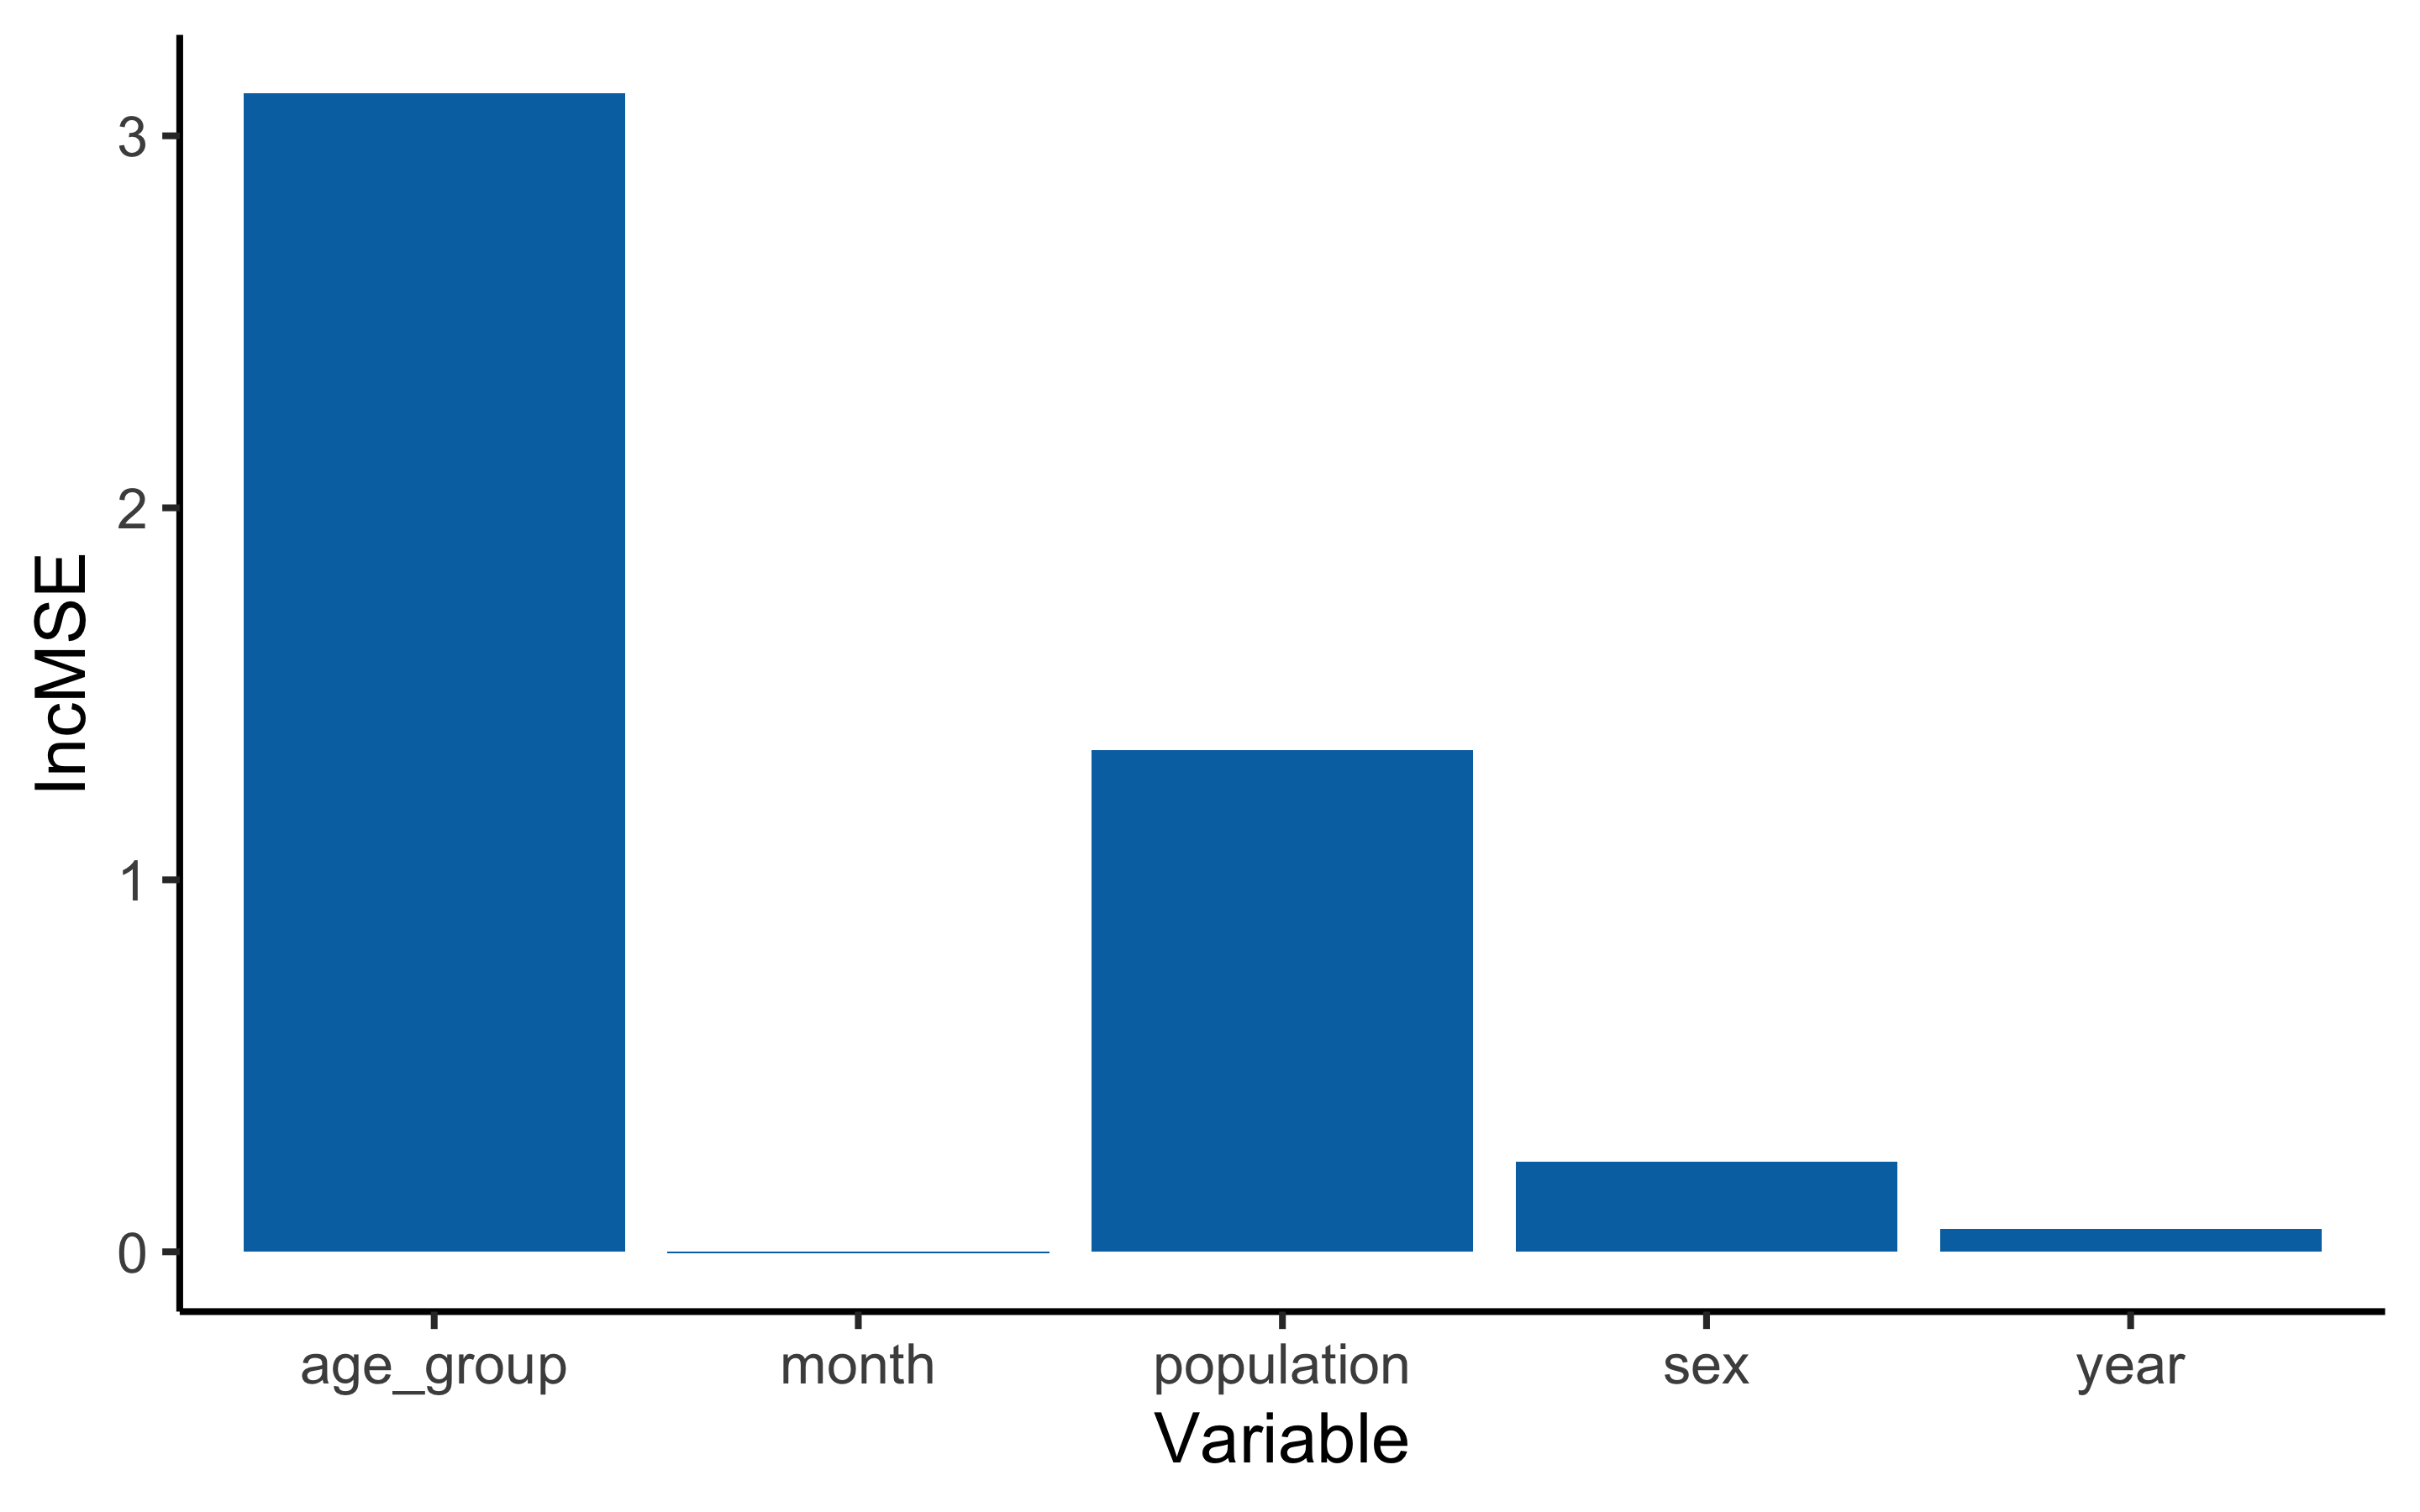
\includegraphics[scale=0.075]{figs/rf_plot.png}
\caption{Variable importance plot}
\label{fig:rf_imp}
\end{subfigure}
\begin{subfigure}[t]{0.49\textwidth}
\centering
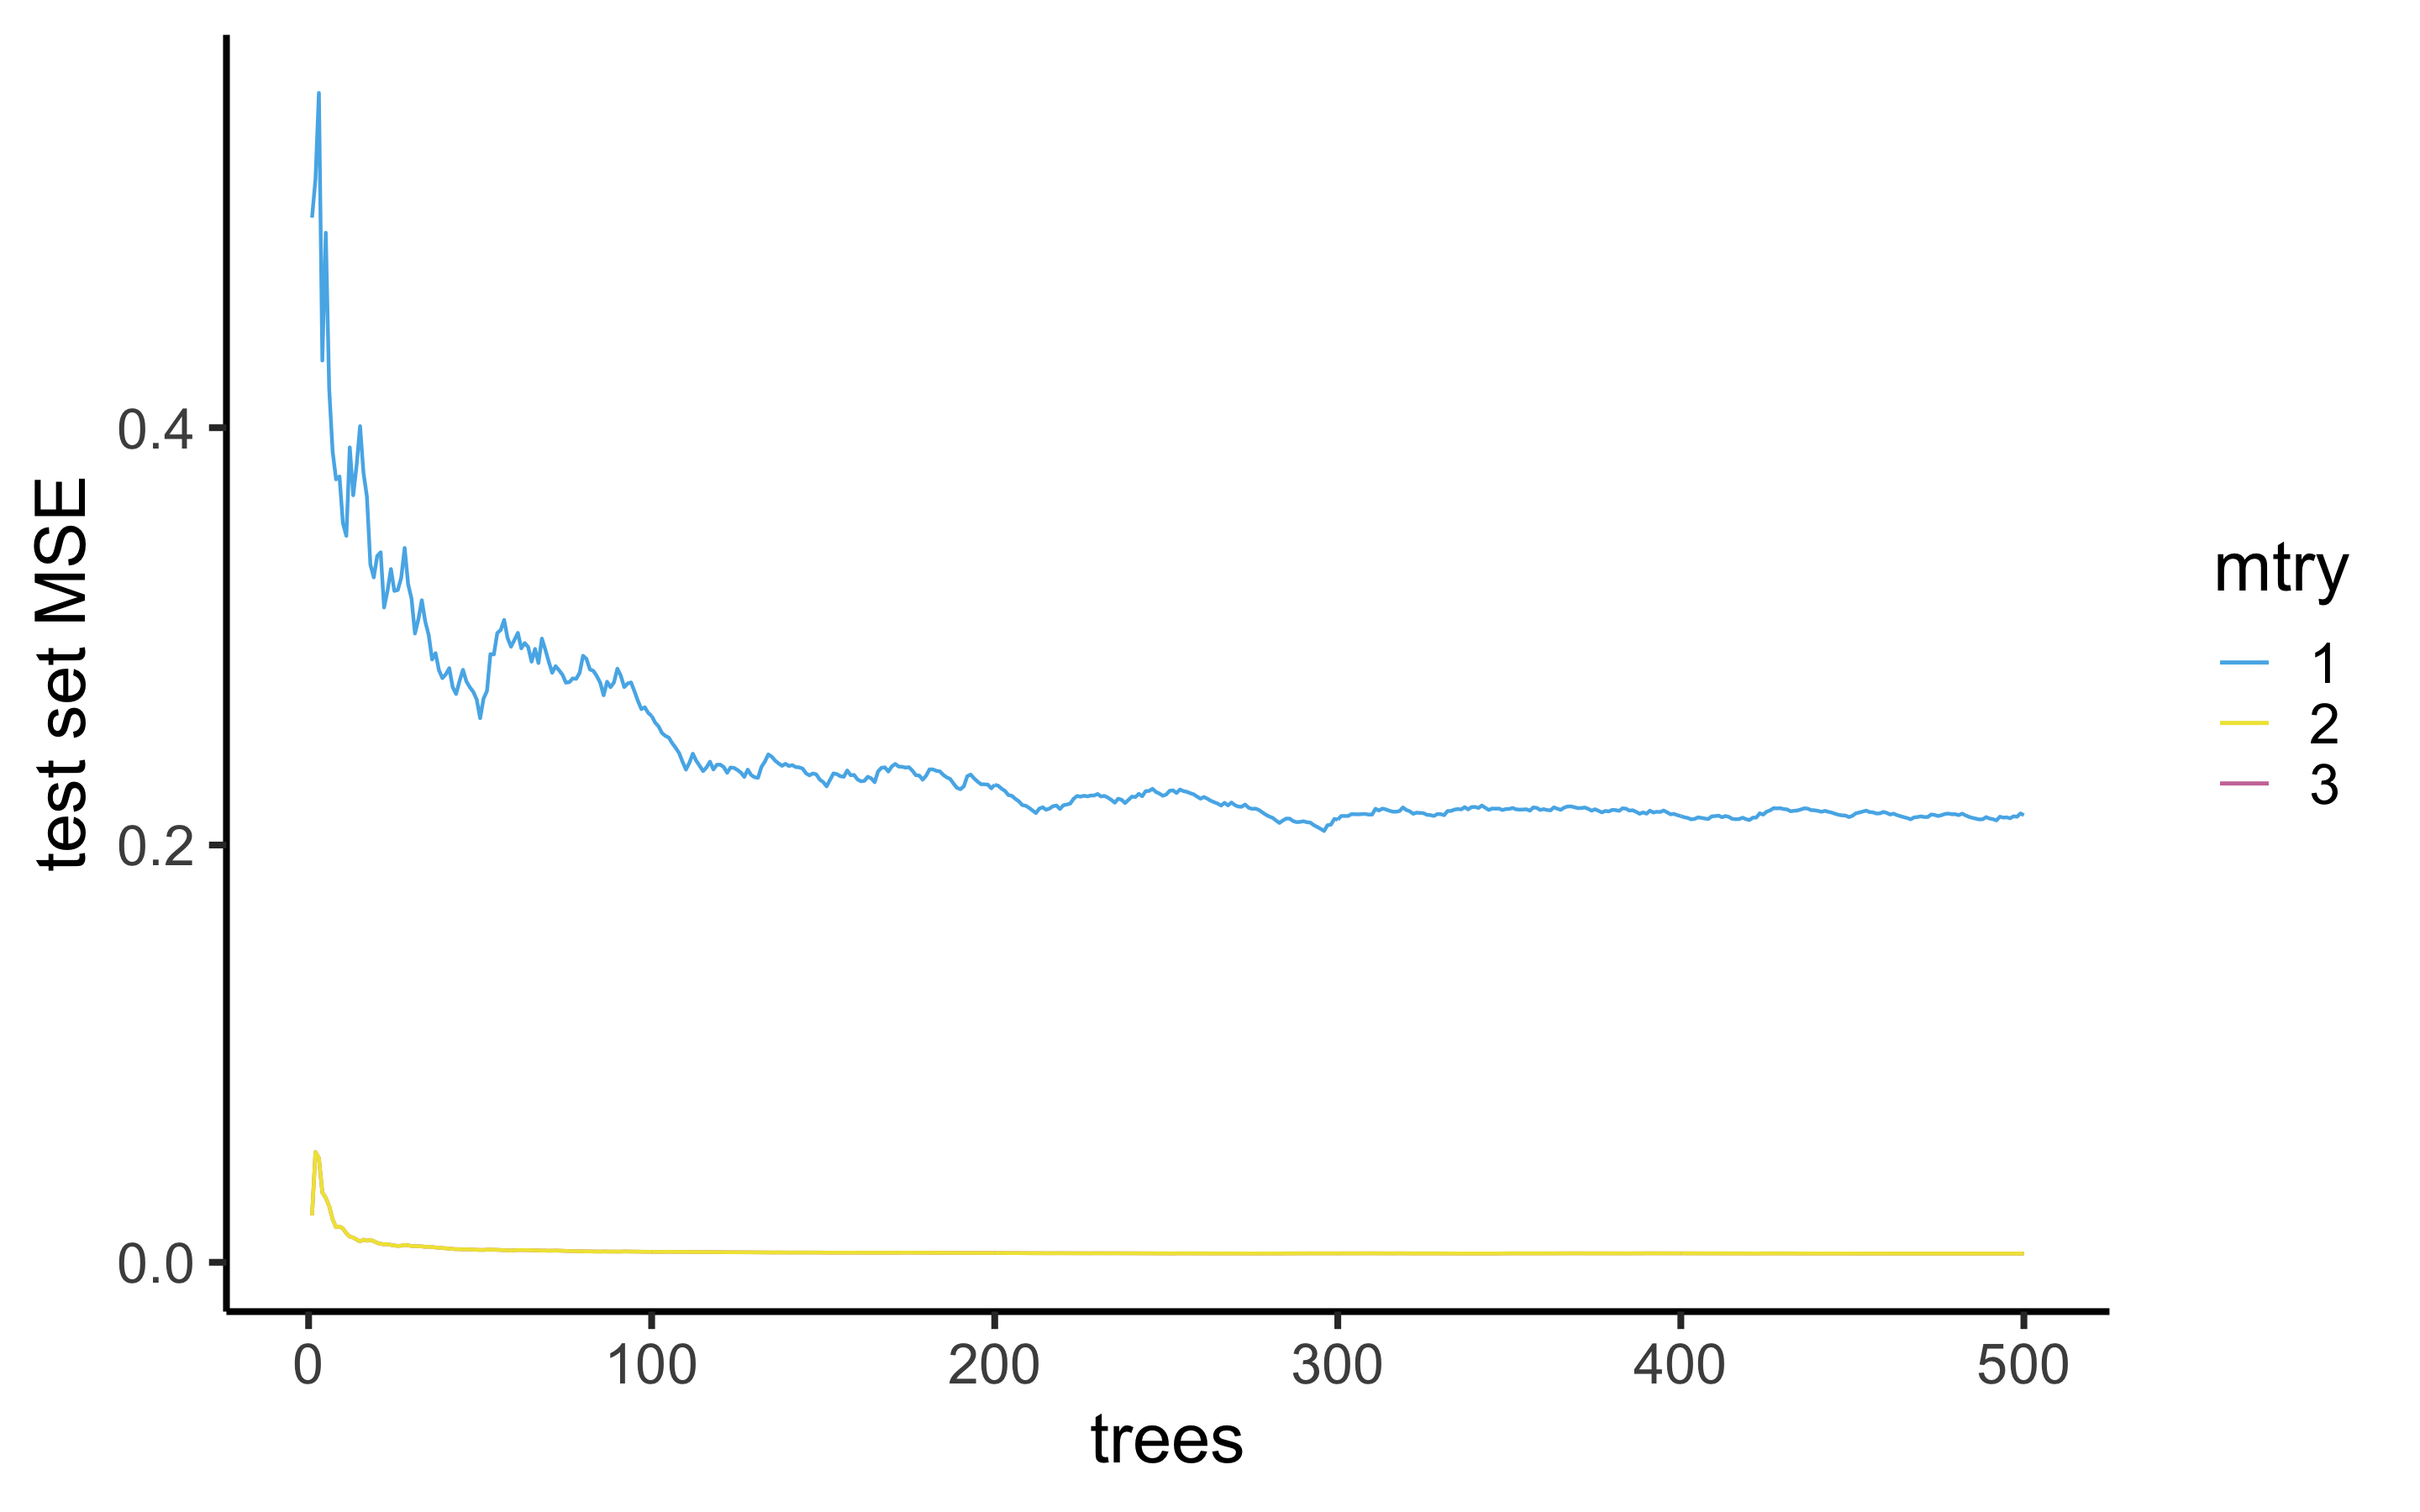
\includegraphics[scale=0.075]{figs/rf_err_plot.png}
\caption{Test error plot}
\label{fig:rf_err}
\end{subfigure}
\caption{Random forest plots}
\label{rf_plots}
\end{figure}

While the random forest can't tell us which interactions are significant, we can use the variable importance plot in \cref{fig:rf_imp} to see which variables, in general, are significant for determining mortality rate.
The importance measure is the recorded improvement in the split-criterion (in this case, MSE) accumulated over all the trees for each splitting variable\cite{ESL}.
Our plot shows that the age group is the most important variable, which seems concordant with our inferences in \cref{sec:inference}.
Ignoring the population variable (we included it as a predictor since \verb+randomForest+ does not have an option for offset), the next most important variable is the sex, which again seems to agree with our previous analysis which showed males having a higher death rate than females in every age group.
Finally, we see a small effect from year and a minimal effect from month, though the effect of these variables may be more apparent through their interactions with other variables (such as age).

\subsection{Modeling death counts with a generalized additive model}\label{sec:gam}

The random forest does not, however, indicate the direction or size of these effects, nor can we visualize the interactions between variables, so we fit a generalized additive model (GAM) which will allow us to account for interactions between the variables as well as nonlinearity between the death rate and covariates.
A GAM models nonlinear regression effects by taking the sum of smooth functions of the predictors, and we can estimate different curves for a continuous variable (i.e., year) for each level of a factor variable (i.e., age)\cite{ESL}.

Since the most successful model in \cref{sec:poisson} included interactions between age and month as well as age and year, we want to account for those in our additive model.
Using the \verb+mgcv+ implementation in R\cite{mgcv}, we fit a GAM in the quasipoisson family that included main effects for \verb+sex+ and \verb+age_group+, an offset for \verb+log(population)+,
and smooth functions for month and year, both evaluated for each level of the factor variable \verb+age_group+. 
The spline for \verb+month+ is a cyclic cubic spline, which enforces a smoothness condition between the first and last months, which seems reasonable given our hypothesis that the winter months result in higher deaths for seniors and December and January should have similar effects.

\begin{figure}
\centering
\begin{subfigure}[t]{0.32\textwidth}
\centering
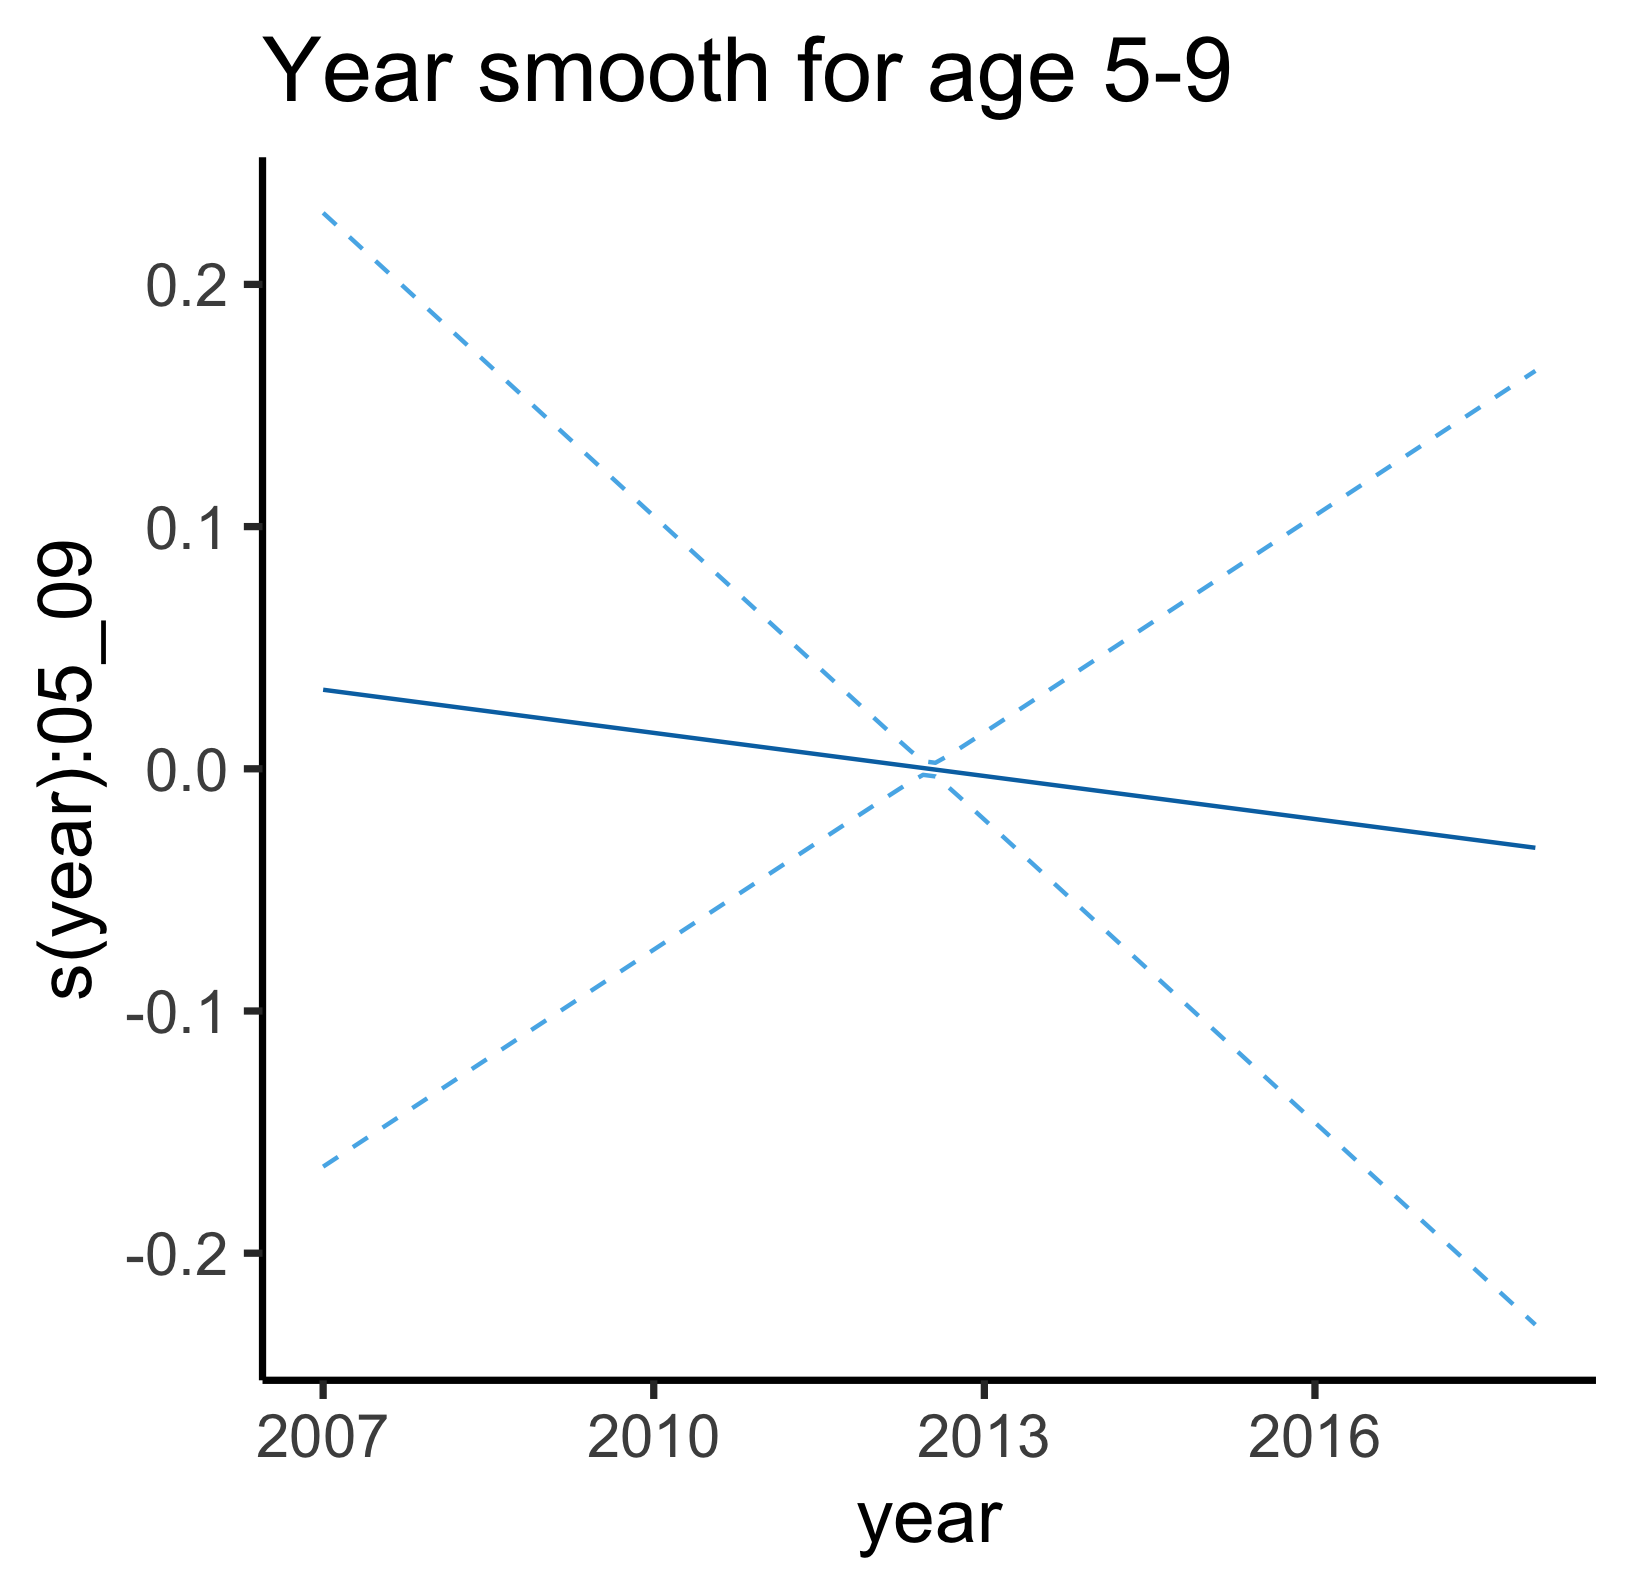
\includegraphics[scale=0.077]{figs/gam_plot4.png}
\caption{Fitted curve  for ages 5-9}
\label{fig:gam_plot4}
\end{subfigure}
\begin{subfigure}[t]{0.32\textwidth}
\centering
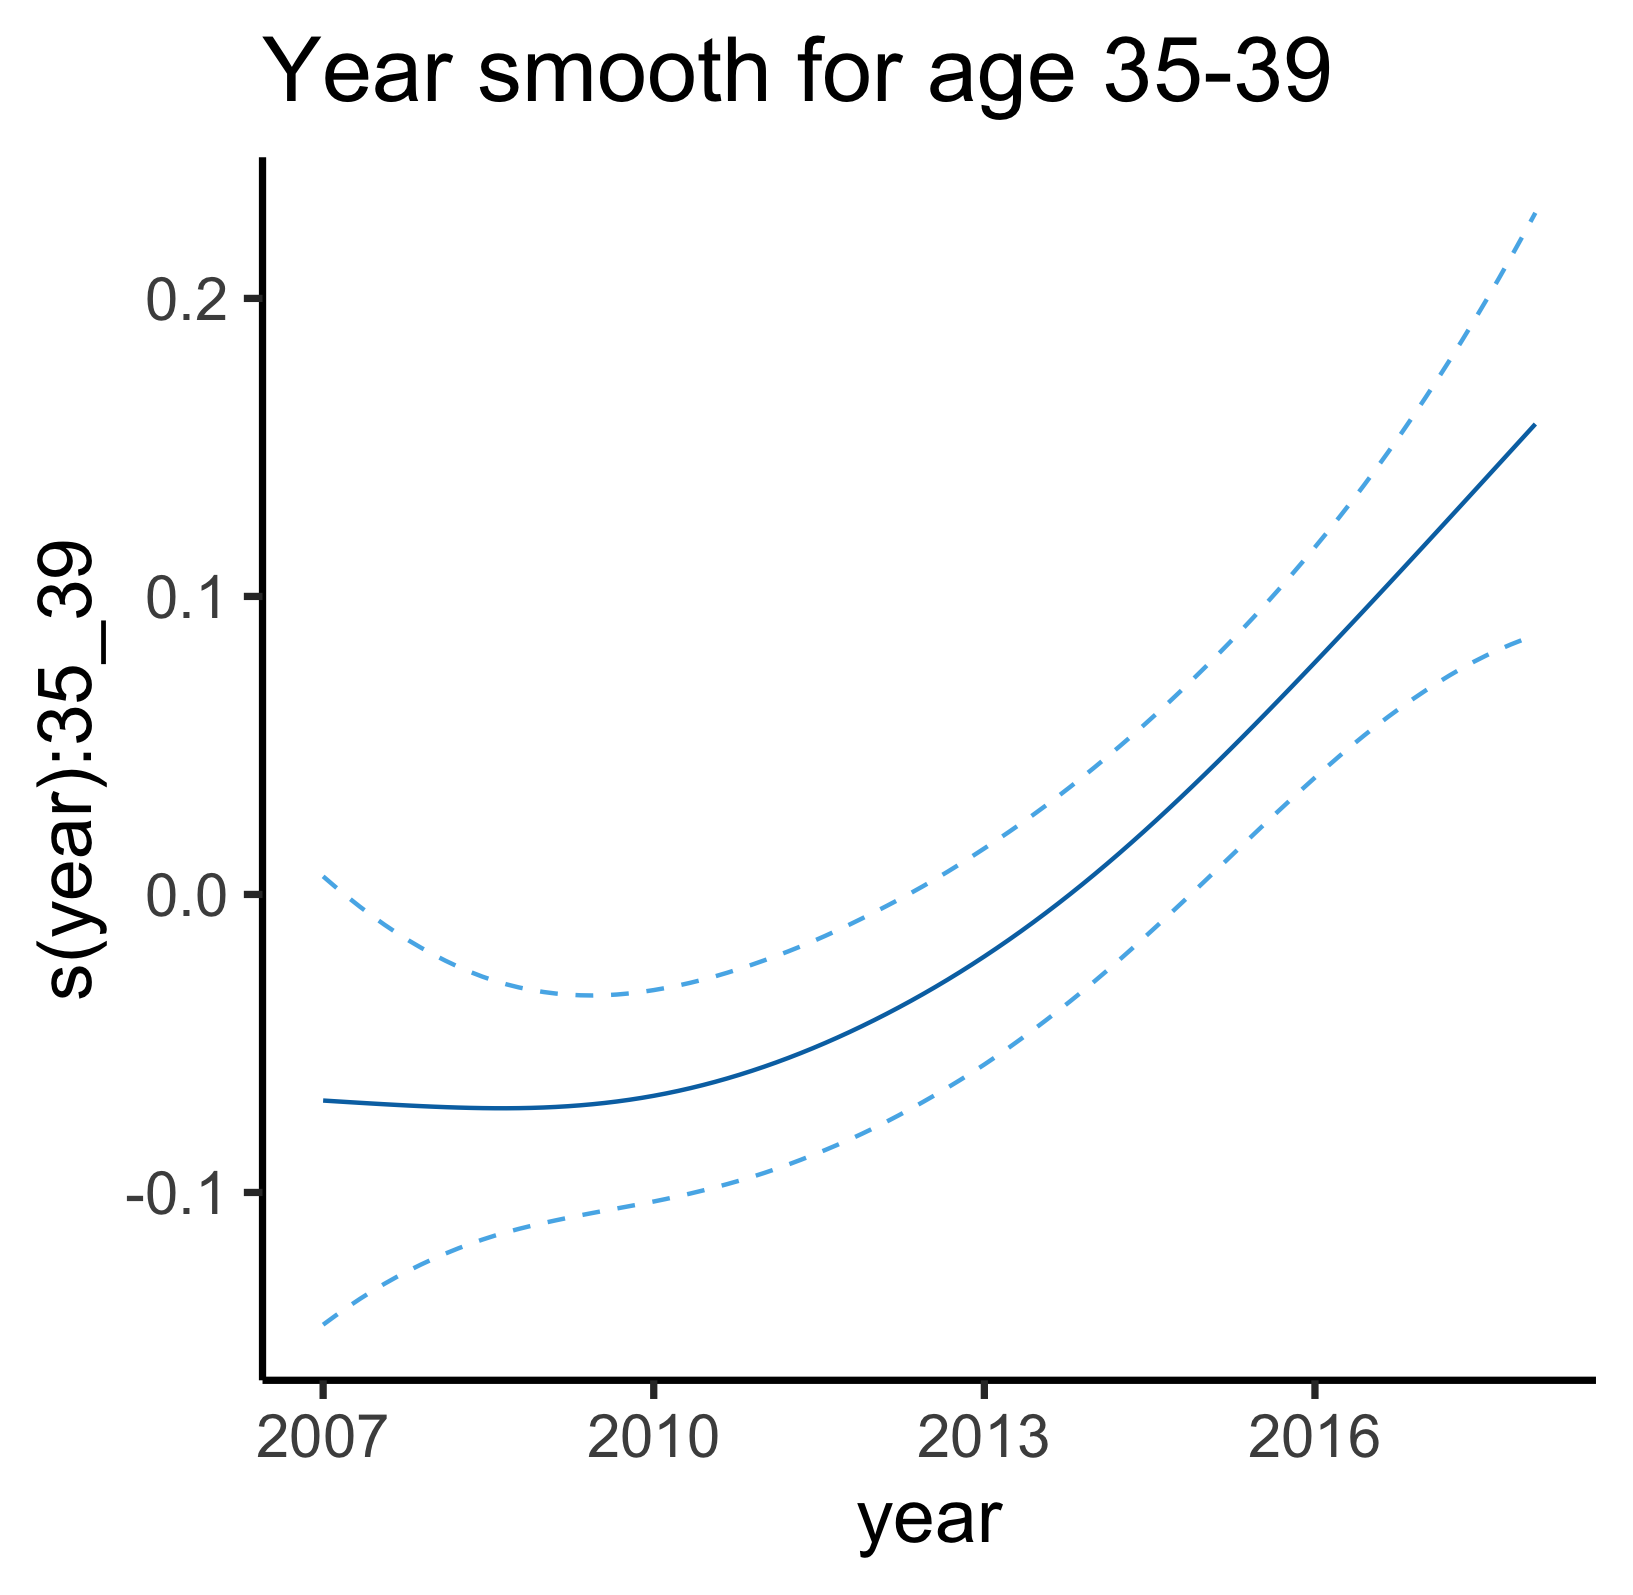
\includegraphics[scale=0.077]{figs/gam_plot5.png}
\caption{Fitted curve  for ages 35-39}
\label{fig:gam_plot5}
\end{subfigure}
\begin{subfigure}[t]{0.32\textwidth}
\centering
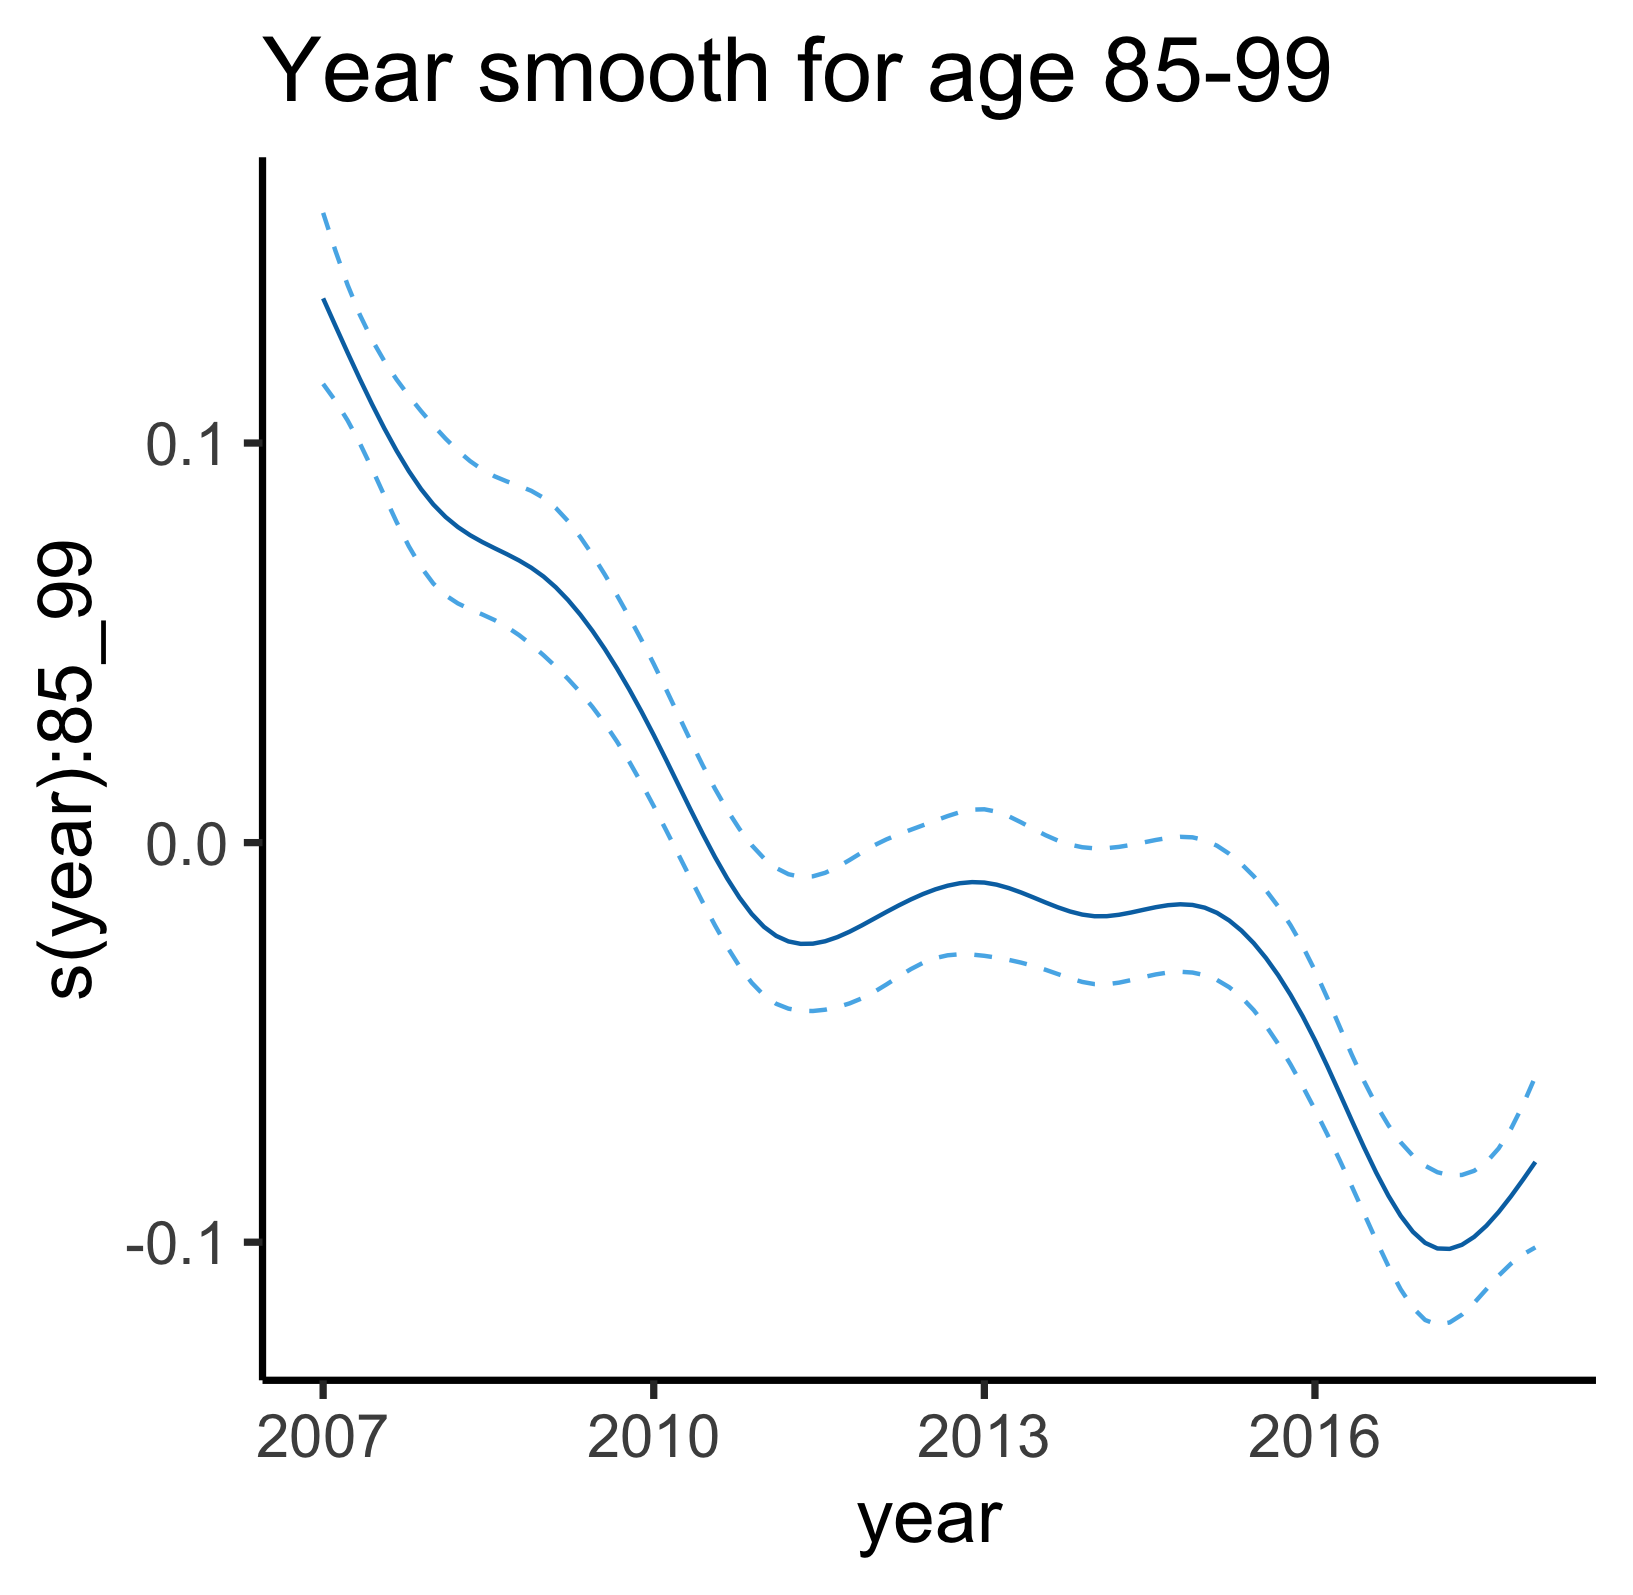
\includegraphics[scale=0.077]{figs/gam_plot6.png}
\caption{Fitted curve for ages 85-99}
\label{fig:gam_plot6}
\end{subfigure}
\caption{Fitted smooth curves for year effect}
\label{fig:gam_year}
\end{figure} 

Our model can be examined visually (using use the \verb+mgcViz+ package in R\cite{mgcviz}) by looking at marginal effects plots that show the fitted smooth functions (with 95\% confidence bounds) for \verb+month+ and \verb+year+ at each level of \verb+age_group+.
We observe year trends in \cref{fig:gam_year}.
First, we note that our observation in \cref{sec:age_year} that young adults/early middle-aged people have seen increasing death rates, when accounting for other variables, indicated by the rising line in \cref{fig:gam_plot5}.
Further, the decline in elderly mortality we observed in \cref{sec:age_year} and \cref{sec:inference} is also apparent in \cref{fig:gam_plot6}, where the oldest age group shows a nonlinearly decreasing death rate, though the perturbations in the curve may just be noise, or they could correspond to years with particularly bad seasonal viruses (2015 saw a spike in influenza deaths \cite{cdc_flu}).
Finally, we show little to no trend among young people aged 5-9, which is consistent with our previous results of no significant change in mortality over the last 12 years for children.

\begin{figure}
\centering
\begin{subfigure}[t]{0.32\textwidth}
\centering
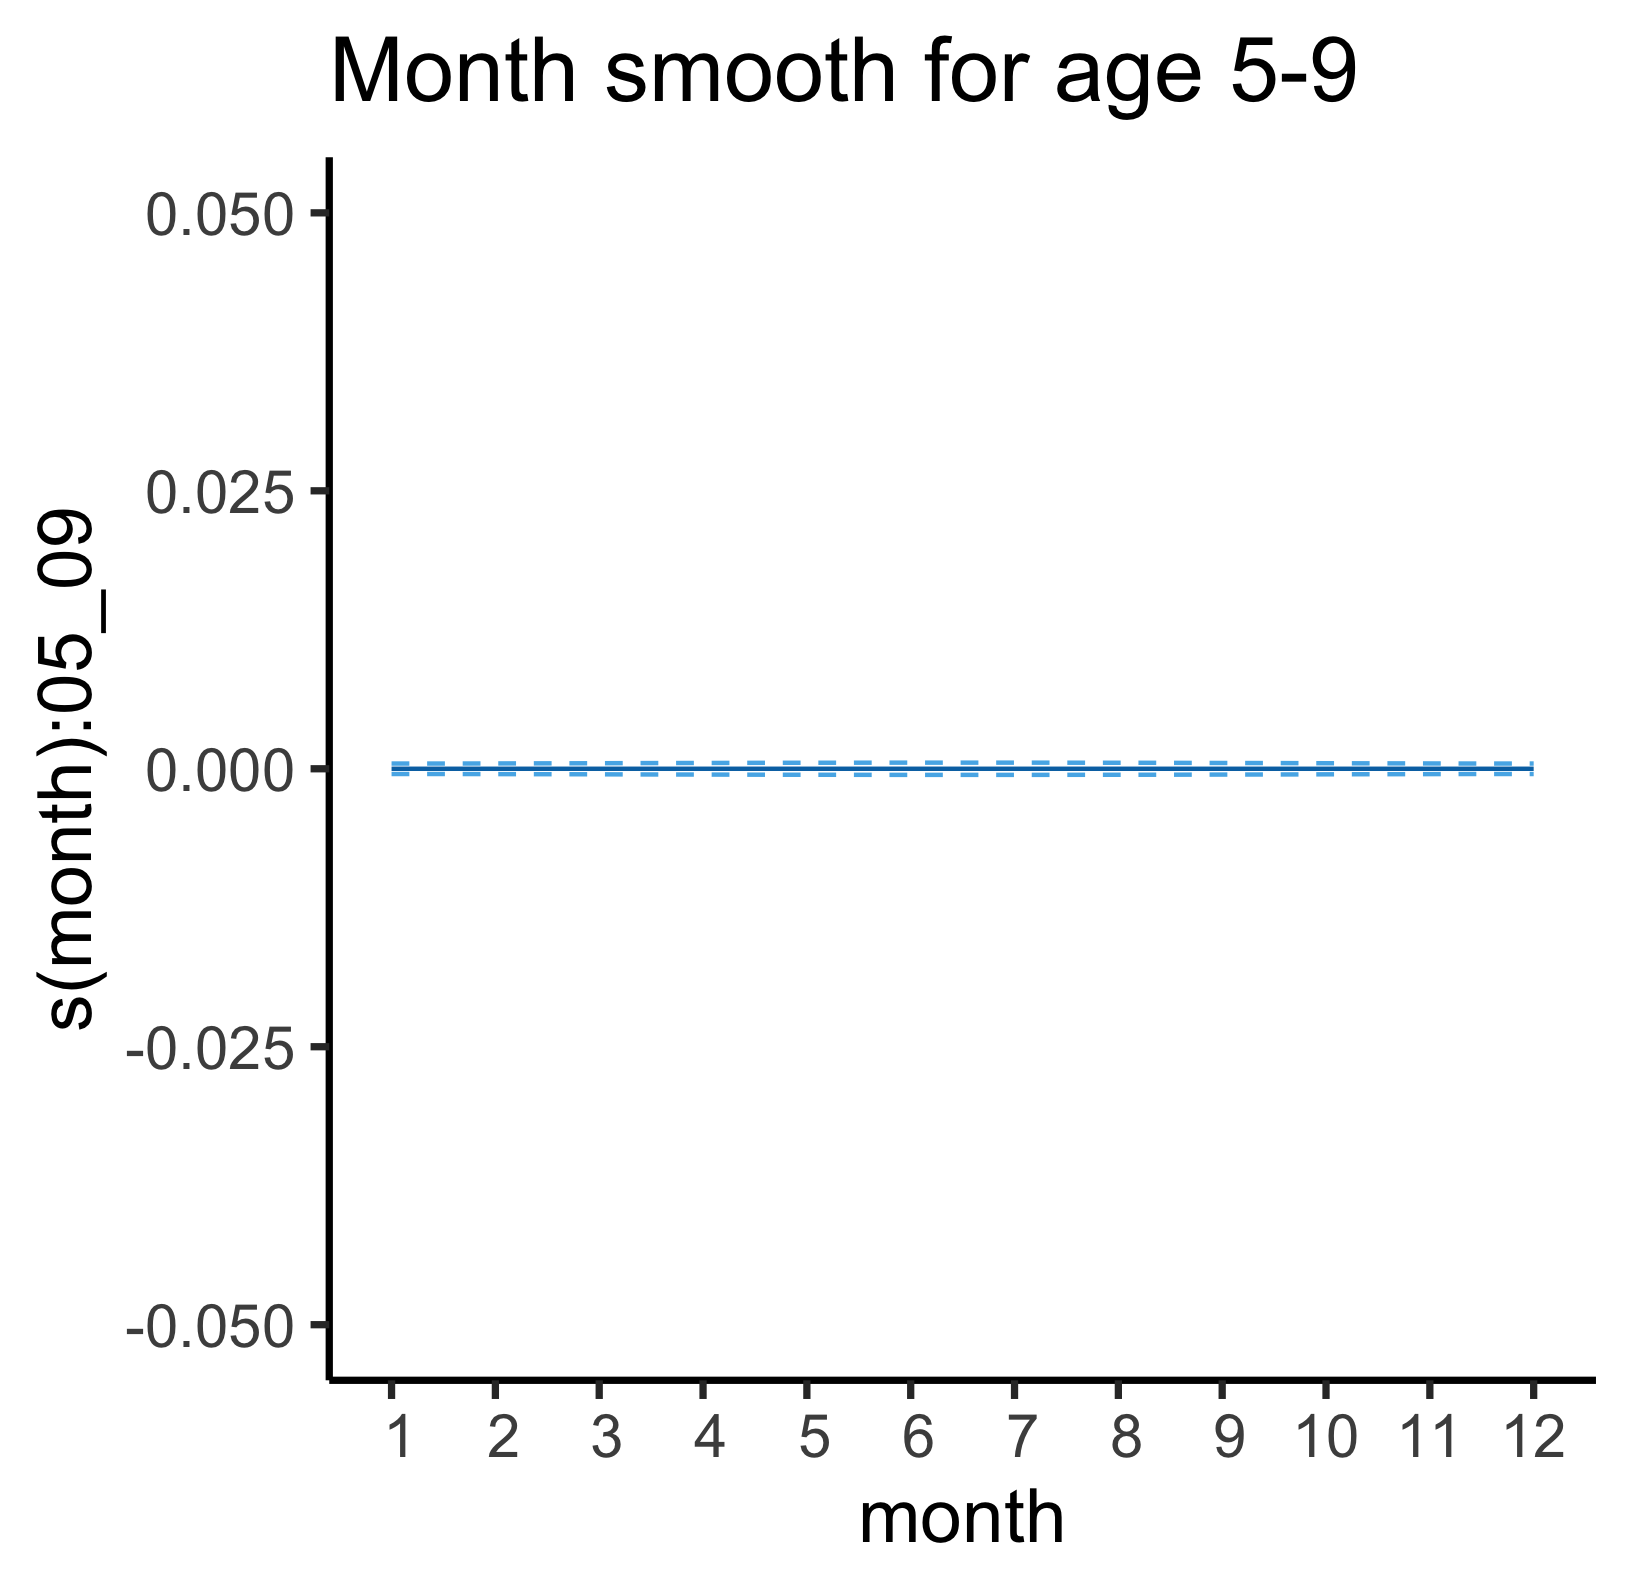
\includegraphics[scale=0.077]{figs/gam_plot1.png}
\caption{Fitted curve for ages 5-9}
\label{fig:gam_plot1}
\end{subfigure}
\begin{subfigure}[t]{0.32\textwidth}
\centering
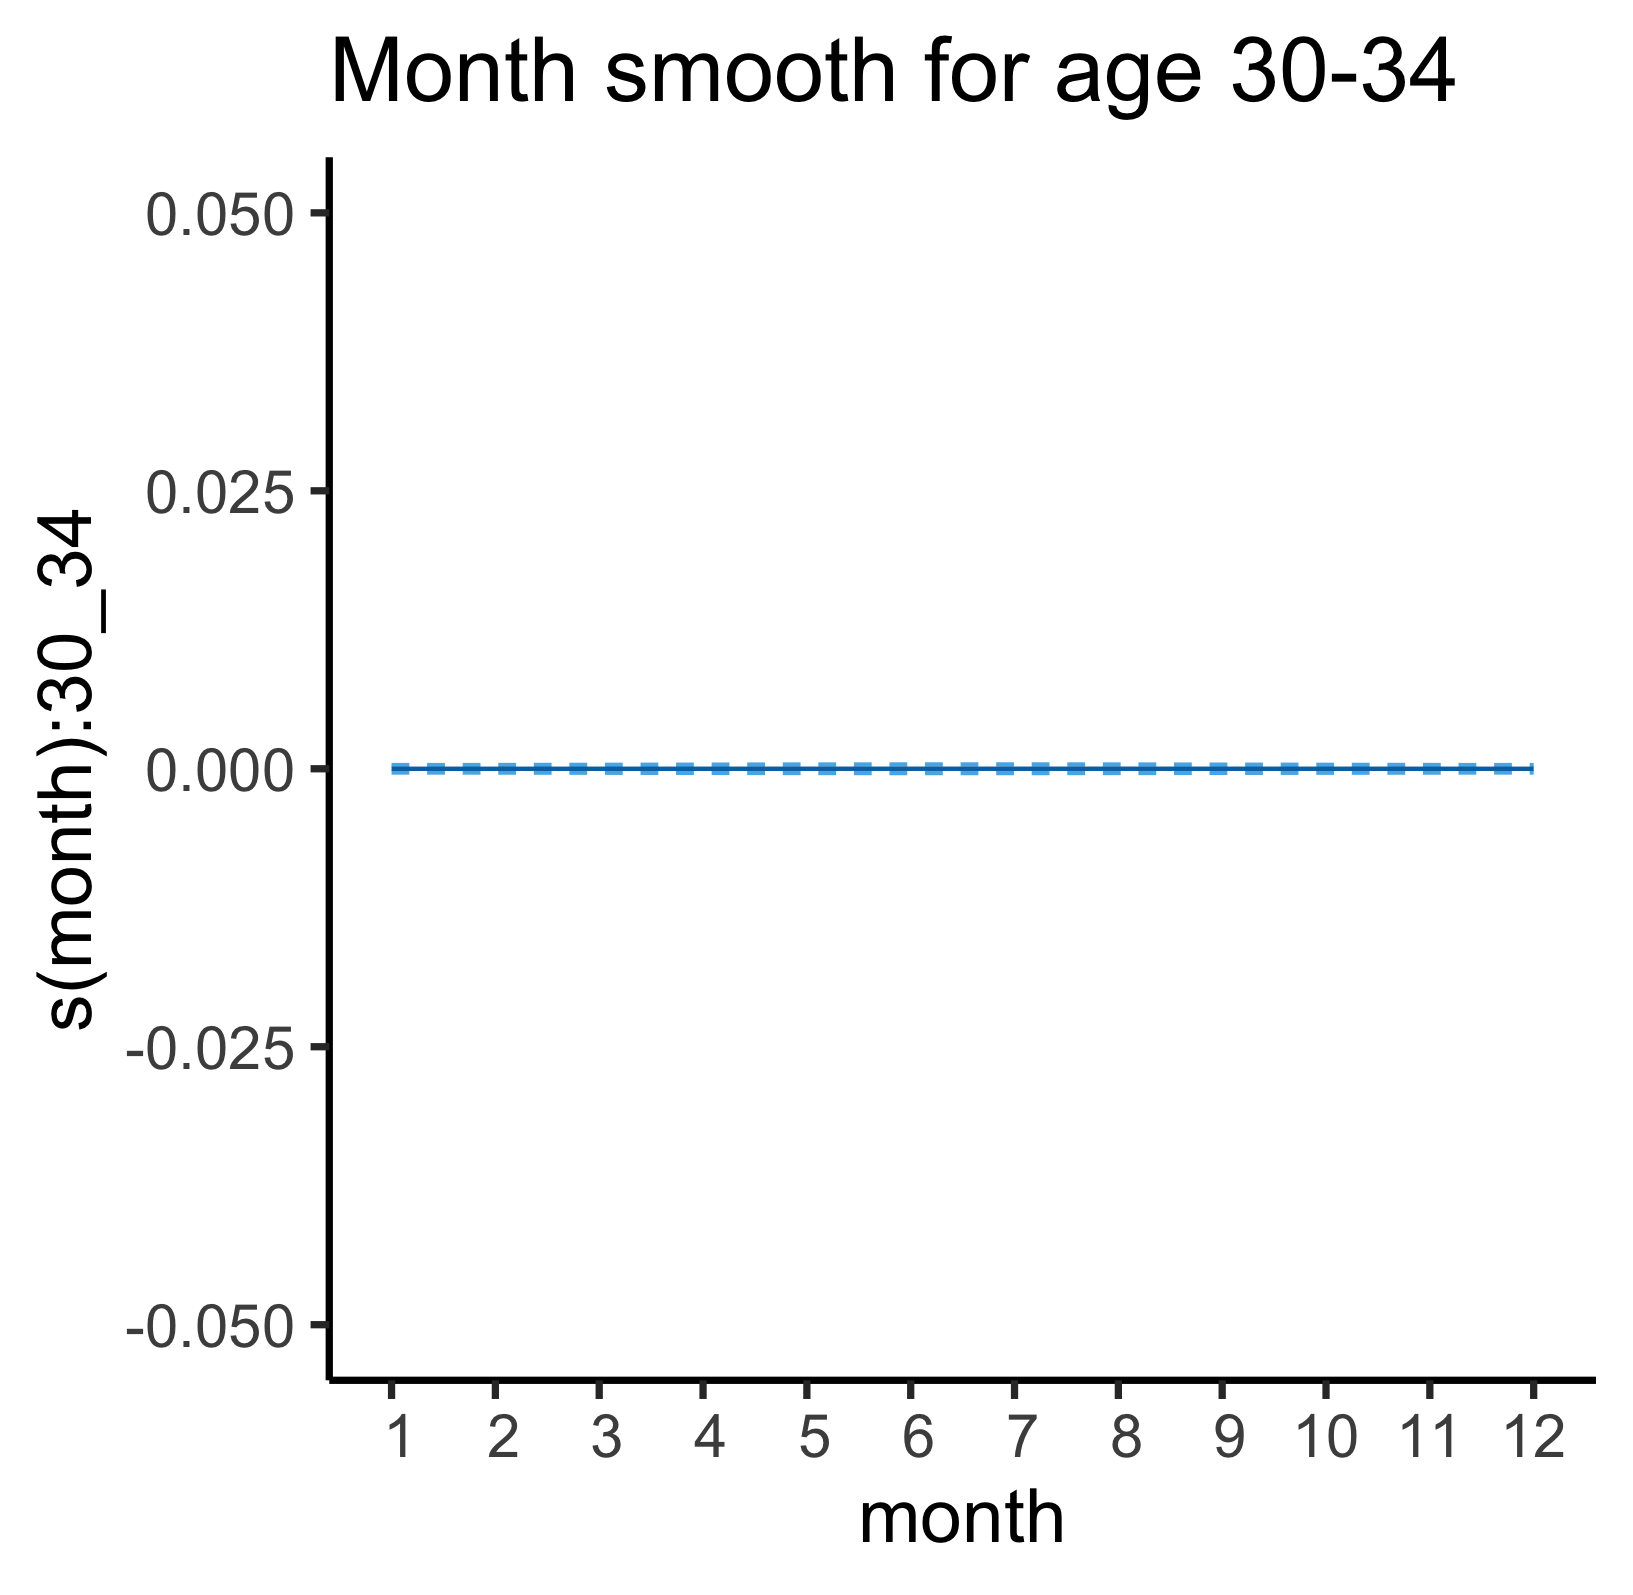
\includegraphics[scale=0.077]{figs/gam_plot2.png}
\caption{Fitted curve for ages 30-34}
\label{fig:gam_plot2}
\end{subfigure}
\begin{subfigure}[t]{0.32\textwidth}
\centering
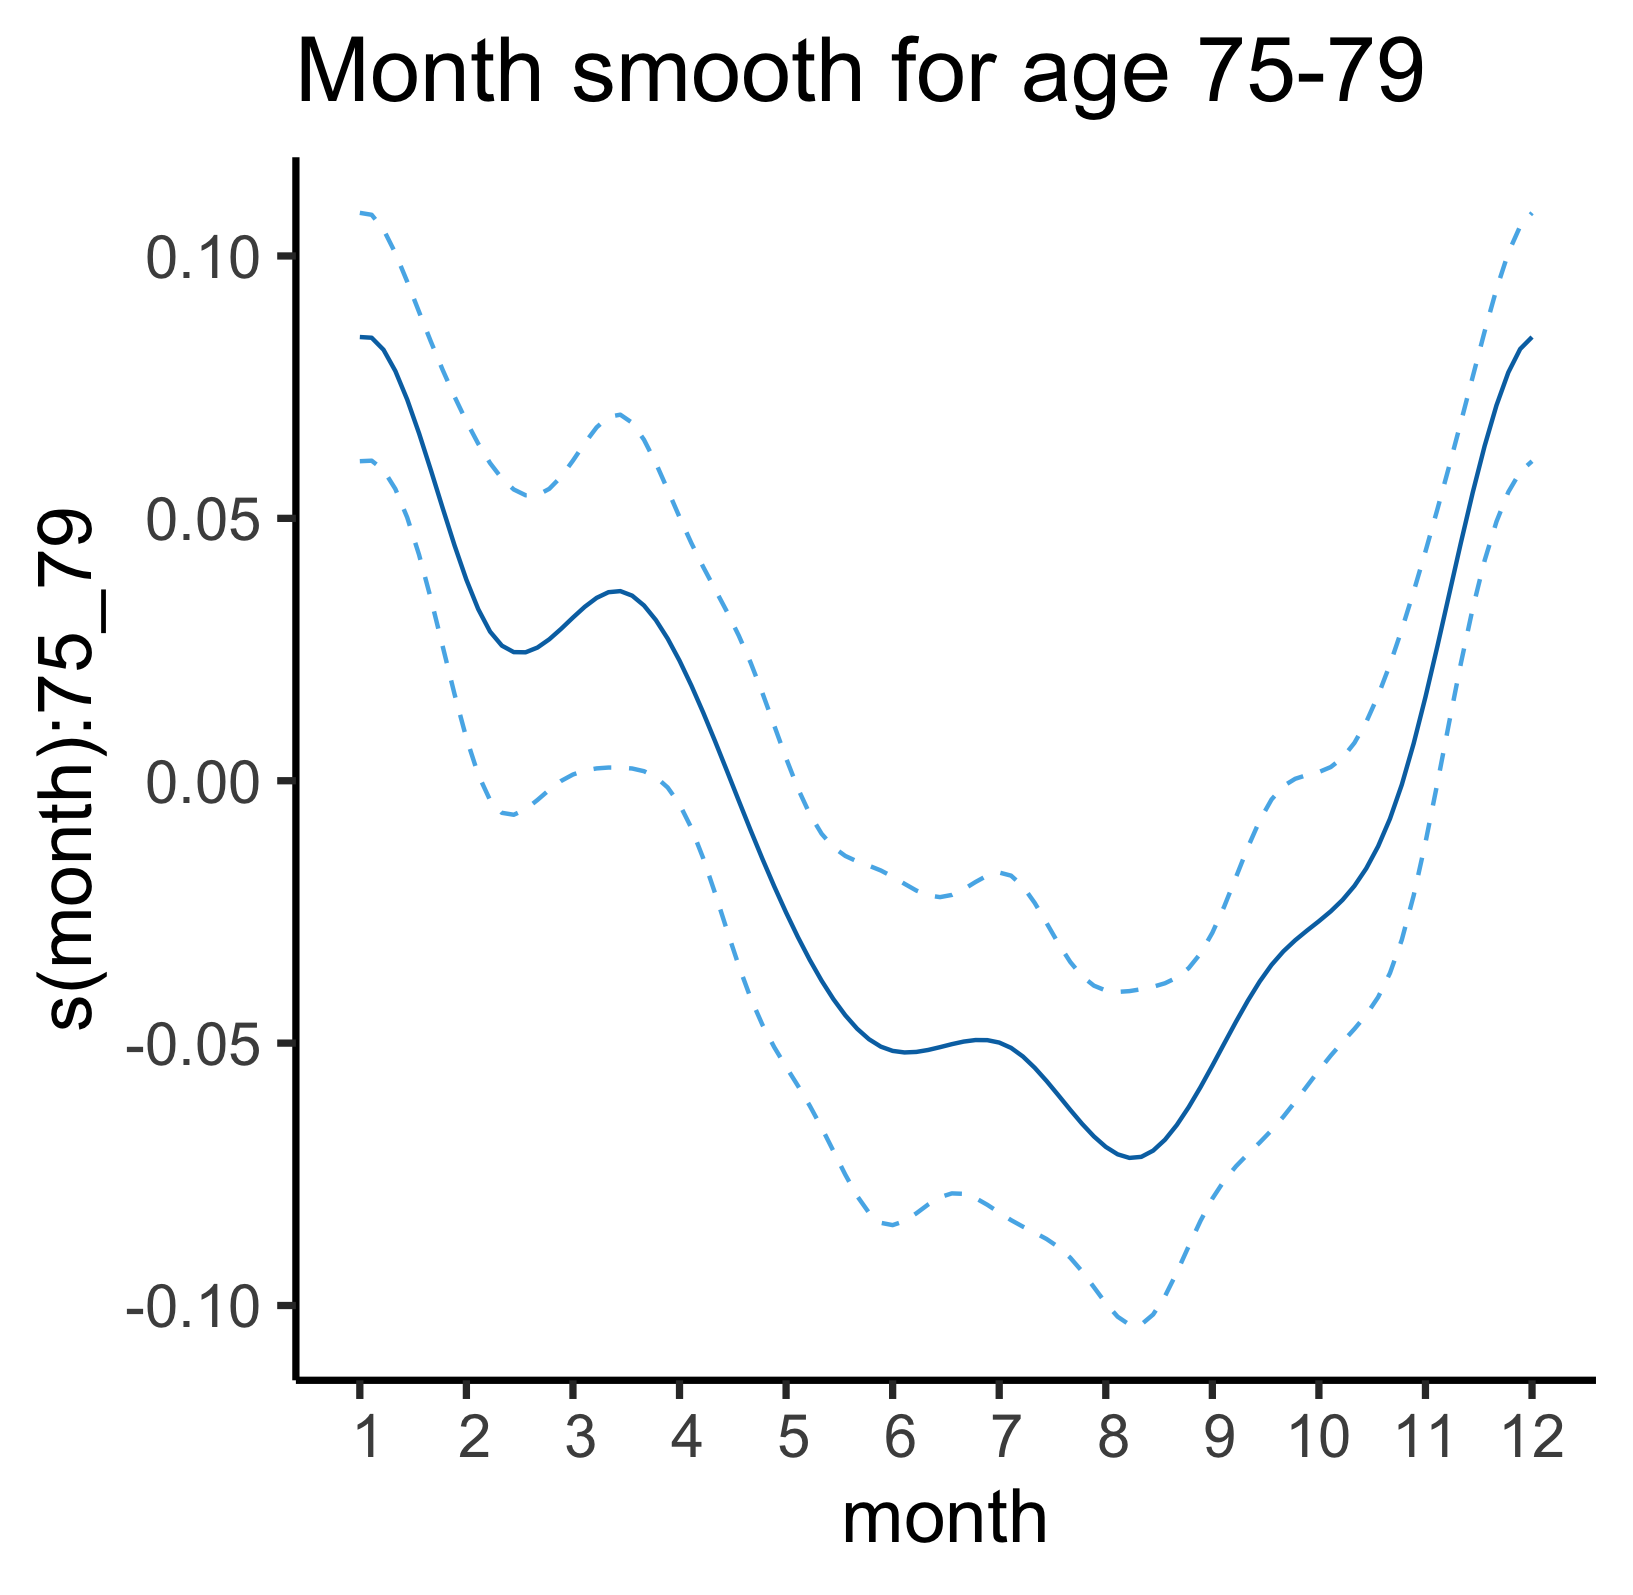
\includegraphics[scale=0.077]{figs/gam_plot3.png}
\caption{Fitted curve for ages 75-79}
\label{fig:gam_plot3}
\end{subfigure}
\caption{Fitted smooth curves for month effect}
\label{fig:gam_month}
\end{figure}

In addition to year-over-year trends in mortality, we can also visualize season trends in mortality from our fitted GAM.
Consistent with our observations in \cref{sec:age_sex}, we note the following trends in seasonal mortality for different age groups. 
The youngest age group, represented in \cref{fig:gam_plot1} by ages 5-9 shows no seasonal trend in mortality. 
We see a slight rise in mortality in the summer months for people aged 30-34 in \cref{fig:gam_plot2}, which is consistent with the rise we saw in the 30-44 age group in \cref{fig:young_men}.
Our intuition about the elderly being susceptible to illnesses in the winter months seems to agree with the trend in \cref{fig:gam_plot3}, which shows significantly higher mortality among those aged 75-79 in the winter months. 

\section{Conclusion and Limitations}\label{sec:conclusion}

Using generalized linear models, random forests, and generalized additive models, we note the following trends in mortality in the U.S. between 2008 and 2017.
\begin{itemize}
\item Males, on average, have a higher death rate than females, and older people, on average, have a much higher death rate than younger people. \vspace{-1mm}
\item Death rates for older people are higher in the winter, whereas for young adults/middle-aged people, death rates are slightly higher in the summer months\vspace{-1mm}
\item Death rates for the elderly, especially those in the 85+ age group have fallen over the last 12 years, while death rates for those in the 30-44 age range have been rising since 2013 and in general have a nonlinear association with year\vspace{-1mm}
\end{itemize}
We stress that these are \textit{average} trends, and a fruitful area of research could be to explore more fine-grained data to see where these trends break down, or where they are accentuated. 
Further, while some explanations for these trends may seem obvious (the elderly are more susceptible to viral infections in the winter such as influenza), others require further research for a satisfying explanation (as in \cite{case2015}).

One major limitation of our analysis is that we are not explicitly modeling time-based dependence in the data. 
Though data for two adjacent months are probably more strongly correlated than data that are many months apart, our models do not incorporate this temporal structure. 
A promising further research direction would be to model these data in a way that takes this serial dependence into account.

Another way to modify our analysis would be to estimate a coefficient for the population of each demographic cell, rather than using an offset.
The offset can be thought of as including a coefficient for \verb+population+ in the model but forcing its value to be 1. 
We could instead just include \verb+population+ as another variable in the model and \textit{estimate} its coefficient.
We should also point out that the population is only computed yearly, while the death count data is reported on a monthly basis. 
Therefore, the death rates are not exact, as the denominator does not update, and death rates in December are probably not as accurate at those in January.

While it will certainly be difficult for the U.S. to repeat the tremendous improvements in public health and decline in mortality rates seen in the 20th century, our report highlights both causes for celebration (continued decrease in mortality for the elderly and infants) and opportunities for improvement (rising mortality among the early middle-aged).
We hope our research can be a starting point for public health experts and medical professionals to continue searching for ways to reduce mortality and increase quality of life for all Americans.

All code used to prepare this analysis can be found at: 

%------------------------------
\newpage
\bibliographystyle{plain}
\bibliography{references}{}

\end{document}
_{•}